% Options for packages loaded elsewhere
\PassOptionsToPackage{unicode}{hyperref}
\PassOptionsToPackage{hyphens}{url}
%
\documentclass[
]{article}
\title{Areal Data Group Project}
\author{Kayla, Ingmar, Hanmo}
\date{2021-12-06}

\usepackage{amsmath,amssymb}
\usepackage{lmodern}
\usepackage{iftex}
\ifPDFTeX
  \usepackage[T1]{fontenc}
  \usepackage[utf8]{inputenc}
  \usepackage{textcomp} % provide euro and other symbols
\else % if luatex or xetex
  \usepackage{unicode-math}
  \defaultfontfeatures{Scale=MatchLowercase}
  \defaultfontfeatures[\rmfamily]{Ligatures=TeX,Scale=1}
\fi
% Use upquote if available, for straight quotes in verbatim environments
\IfFileExists{upquote.sty}{\usepackage{upquote}}{}
\IfFileExists{microtype.sty}{% use microtype if available
  \usepackage[]{microtype}
  \UseMicrotypeSet[protrusion]{basicmath} % disable protrusion for tt fonts
}{}
\makeatletter
\@ifundefined{KOMAClassName}{% if non-KOMA class
  \IfFileExists{parskip.sty}{%
    \usepackage{parskip}
  }{% else
    \setlength{\parindent}{0pt}
    \setlength{\parskip}{6pt plus 2pt minus 1pt}}
}{% if KOMA class
  \KOMAoptions{parskip=half}}
\makeatother
\usepackage{xcolor}
\IfFileExists{xurl.sty}{\usepackage{xurl}}{} % add URL line breaks if available
\IfFileExists{bookmark.sty}{\usepackage{bookmark}}{\usepackage{hyperref}}
\hypersetup{
  pdftitle={Areal Data Group Project},
  pdfauthor={Kayla, Ingmar, Hanmo},
  hidelinks,
  pdfcreator={LaTeX via pandoc}}
\urlstyle{same} % disable monospaced font for URLs
\usepackage[margin=1in]{geometry}
\usepackage{color}
\usepackage{fancyvrb}
\newcommand{\VerbBar}{|}
\newcommand{\VERB}{\Verb[commandchars=\\\{\}]}
\DefineVerbatimEnvironment{Highlighting}{Verbatim}{commandchars=\\\{\}}
% Add ',fontsize=\small' for more characters per line
\usepackage{framed}
\definecolor{shadecolor}{RGB}{248,248,248}
\newenvironment{Shaded}{\begin{snugshade}}{\end{snugshade}}
\newcommand{\AlertTok}[1]{\textcolor[rgb]{0.94,0.16,0.16}{#1}}
\newcommand{\AnnotationTok}[1]{\textcolor[rgb]{0.56,0.35,0.01}{\textbf{\textit{#1}}}}
\newcommand{\AttributeTok}[1]{\textcolor[rgb]{0.77,0.63,0.00}{#1}}
\newcommand{\BaseNTok}[1]{\textcolor[rgb]{0.00,0.00,0.81}{#1}}
\newcommand{\BuiltInTok}[1]{#1}
\newcommand{\CharTok}[1]{\textcolor[rgb]{0.31,0.60,0.02}{#1}}
\newcommand{\CommentTok}[1]{\textcolor[rgb]{0.56,0.35,0.01}{\textit{#1}}}
\newcommand{\CommentVarTok}[1]{\textcolor[rgb]{0.56,0.35,0.01}{\textbf{\textit{#1}}}}
\newcommand{\ConstantTok}[1]{\textcolor[rgb]{0.00,0.00,0.00}{#1}}
\newcommand{\ControlFlowTok}[1]{\textcolor[rgb]{0.13,0.29,0.53}{\textbf{#1}}}
\newcommand{\DataTypeTok}[1]{\textcolor[rgb]{0.13,0.29,0.53}{#1}}
\newcommand{\DecValTok}[1]{\textcolor[rgb]{0.00,0.00,0.81}{#1}}
\newcommand{\DocumentationTok}[1]{\textcolor[rgb]{0.56,0.35,0.01}{\textbf{\textit{#1}}}}
\newcommand{\ErrorTok}[1]{\textcolor[rgb]{0.64,0.00,0.00}{\textbf{#1}}}
\newcommand{\ExtensionTok}[1]{#1}
\newcommand{\FloatTok}[1]{\textcolor[rgb]{0.00,0.00,0.81}{#1}}
\newcommand{\FunctionTok}[1]{\textcolor[rgb]{0.00,0.00,0.00}{#1}}
\newcommand{\ImportTok}[1]{#1}
\newcommand{\InformationTok}[1]{\textcolor[rgb]{0.56,0.35,0.01}{\textbf{\textit{#1}}}}
\newcommand{\KeywordTok}[1]{\textcolor[rgb]{0.13,0.29,0.53}{\textbf{#1}}}
\newcommand{\NormalTok}[1]{#1}
\newcommand{\OperatorTok}[1]{\textcolor[rgb]{0.81,0.36,0.00}{\textbf{#1}}}
\newcommand{\OtherTok}[1]{\textcolor[rgb]{0.56,0.35,0.01}{#1}}
\newcommand{\PreprocessorTok}[1]{\textcolor[rgb]{0.56,0.35,0.01}{\textit{#1}}}
\newcommand{\RegionMarkerTok}[1]{#1}
\newcommand{\SpecialCharTok}[1]{\textcolor[rgb]{0.00,0.00,0.00}{#1}}
\newcommand{\SpecialStringTok}[1]{\textcolor[rgb]{0.31,0.60,0.02}{#1}}
\newcommand{\StringTok}[1]{\textcolor[rgb]{0.31,0.60,0.02}{#1}}
\newcommand{\VariableTok}[1]{\textcolor[rgb]{0.00,0.00,0.00}{#1}}
\newcommand{\VerbatimStringTok}[1]{\textcolor[rgb]{0.31,0.60,0.02}{#1}}
\newcommand{\WarningTok}[1]{\textcolor[rgb]{0.56,0.35,0.01}{\textbf{\textit{#1}}}}
\usepackage{longtable,booktabs,array}
\usepackage{calc} % for calculating minipage widths
% Correct order of tables after \paragraph or \subparagraph
\usepackage{etoolbox}
\makeatletter
\patchcmd\longtable{\par}{\if@noskipsec\mbox{}\fi\par}{}{}
\makeatother
% Allow footnotes in longtable head/foot
\IfFileExists{footnotehyper.sty}{\usepackage{footnotehyper}}{\usepackage{footnote}}
\makesavenoteenv{longtable}
\usepackage{graphicx}
\makeatletter
\def\maxwidth{\ifdim\Gin@nat@width>\linewidth\linewidth\else\Gin@nat@width\fi}
\def\maxheight{\ifdim\Gin@nat@height>\textheight\textheight\else\Gin@nat@height\fi}
\makeatother
% Scale images if necessary, so that they will not overflow the page
% margins by default, and it is still possible to overwrite the defaults
% using explicit options in \includegraphics[width, height, ...]{}
\setkeys{Gin}{width=\maxwidth,height=\maxheight,keepaspectratio}
% Set default figure placement to htbp
\makeatletter
\def\fps@figure{htbp}
\makeatother
\setlength{\emergencystretch}{3em} % prevent overfull lines
\providecommand{\tightlist}{%
  \setlength{\itemsep}{0pt}\setlength{\parskip}{0pt}}
\setcounter{secnumdepth}{-\maxdimen} % remove section numbering
\newlength{\cslhangindent}
\setlength{\cslhangindent}{1.5em}
\newlength{\csllabelwidth}
\setlength{\csllabelwidth}{3em}
\newlength{\cslentryspacingunit} % times entry-spacing
\setlength{\cslentryspacingunit}{\parskip}
\newenvironment{CSLReferences}[2] % #1 hanging-ident, #2 entry spacing
 {% don't indent paragraphs
  \setlength{\parindent}{0pt}
  % turn on hanging indent if param 1 is 1
  \ifodd #1
  \let\oldpar\par
  \def\par{\hangindent=\cslhangindent\oldpar}
  \fi
  % set entry spacing
  \setlength{\parskip}{#2\cslentryspacingunit}
 }%
 {}
\usepackage{calc}
\newcommand{\CSLBlock}[1]{#1\hfill\break}
\newcommand{\CSLLeftMargin}[1]{\parbox[t]{\csllabelwidth}{#1}}
\newcommand{\CSLRightInline}[1]{\parbox[t]{\linewidth - \csllabelwidth}{#1}\break}
\newcommand{\CSLIndent}[1]{\hspace{\cslhangindent}#1}
\ifLuaTeX
  \usepackage{selnolig}  % disable illegal ligatures
\fi

\begin{document}
\maketitle

{
\setcounter{tocdepth}{3}
\tableofcontents
}
\newpage

\hypertarget{introduction-to-areal-data}{%
\section{Introduction to Areal Data}\label{introduction-to-areal-data}}

Areal data is spatial data which is observed or reported for spatial
units which are polygons with defined borders. Some examples are country
level data, state level data, county level data, or zip code level data
where the data is aggregated for the defined area. This is often the
case for private information (e.g.~mean income in a zip code instead of
income of each individual with their address), or data the is collected
at that scale (e.g.~proportion of democratic voters in an electoral
unit; Bivand et al., 2013).

Some of the common problems we have with areal data have to do with the
selected boundary. For example, gerrymandering is a common issue with
votes because changing the boundaries yields different election results.
Another issue is that the choice of boundaries is often not made for the
specific question being asked in the model. Bivand et al., 2013 gives
the example of zip codes which are a common unit for demographic data to
be reported in, but were designed for postal delivery not demographic
data collection. The boundaries not fitting the underlying patterns in
the data can cause model misspecification, spatial autocorrelation, and
make it difficult to ascertain the number of independent observations in
a dataset. Therefore, it is important to check for spatial patterning
due to this partitioning to see if the model indicated is appropriate
(Bivand et al., 2013).

\hypertarget{neighbors-and-weights}{%
\subsection{Neighbors and weights}\label{neighbors-and-weights}}

Because we do not have a continuous surface on which to calculate
distance between points to build a variogram we must consider neighbors
instead. There are many ways to describe neighbors. Here are a few
examples where we considering the neighbors \(j\) of the center polygon
\(i\) where \(i\) and \(j\) are \(1\dots n_{polygons}\), and the
polygons \(j\) and colored based on if we consider them to be neighbors
or not.

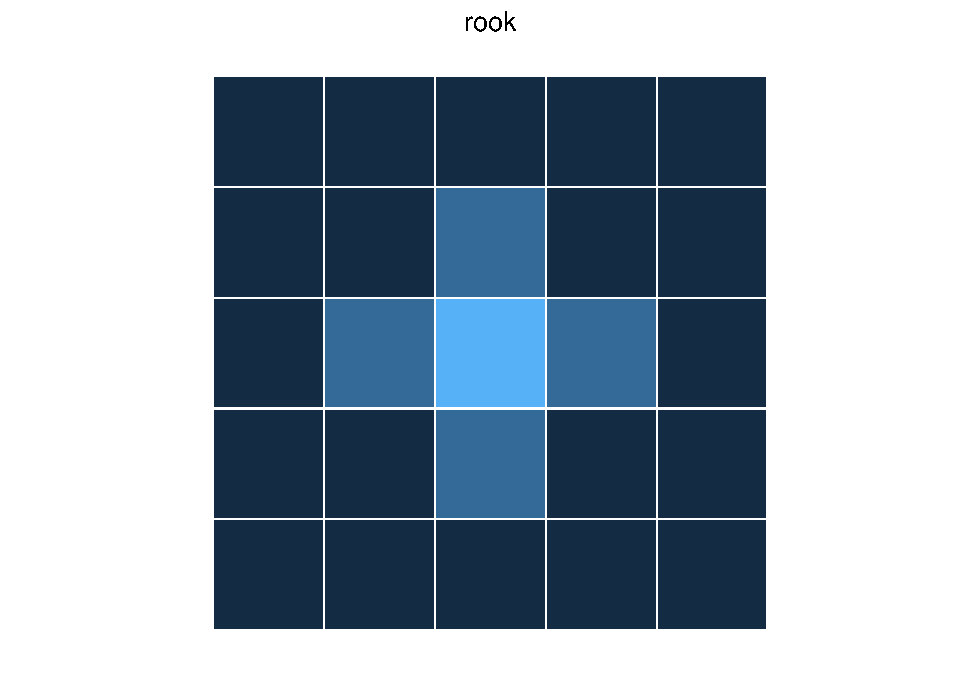
\includegraphics[width=0.25\linewidth]{midterm-project_files/figure-latex/unnamed-chunk-1-1}
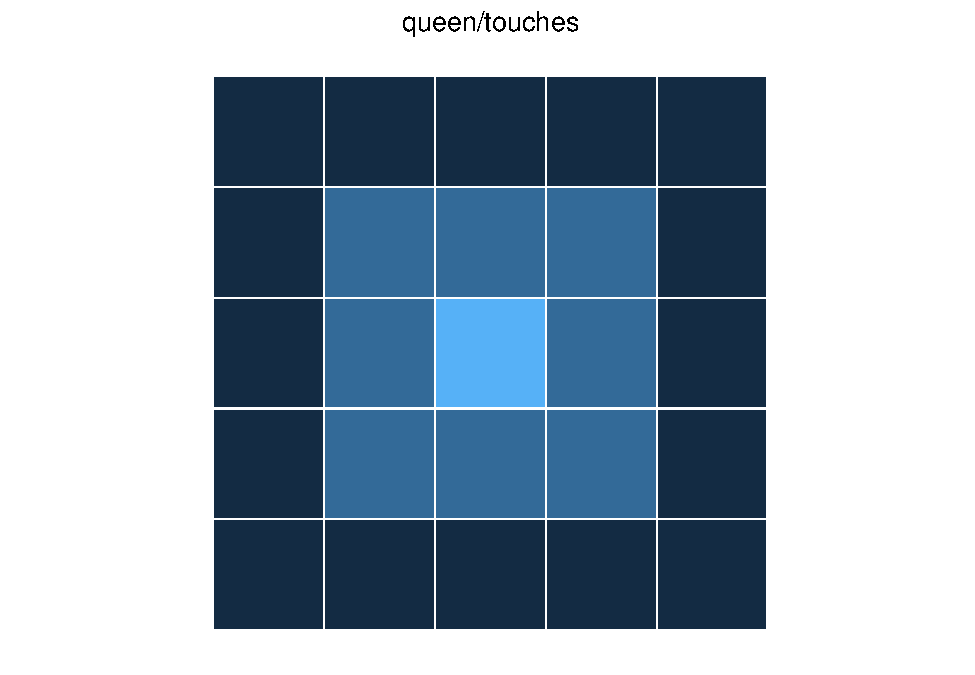
\includegraphics[width=0.25\linewidth]{midterm-project_files/figure-latex/unnamed-chunk-1-2}
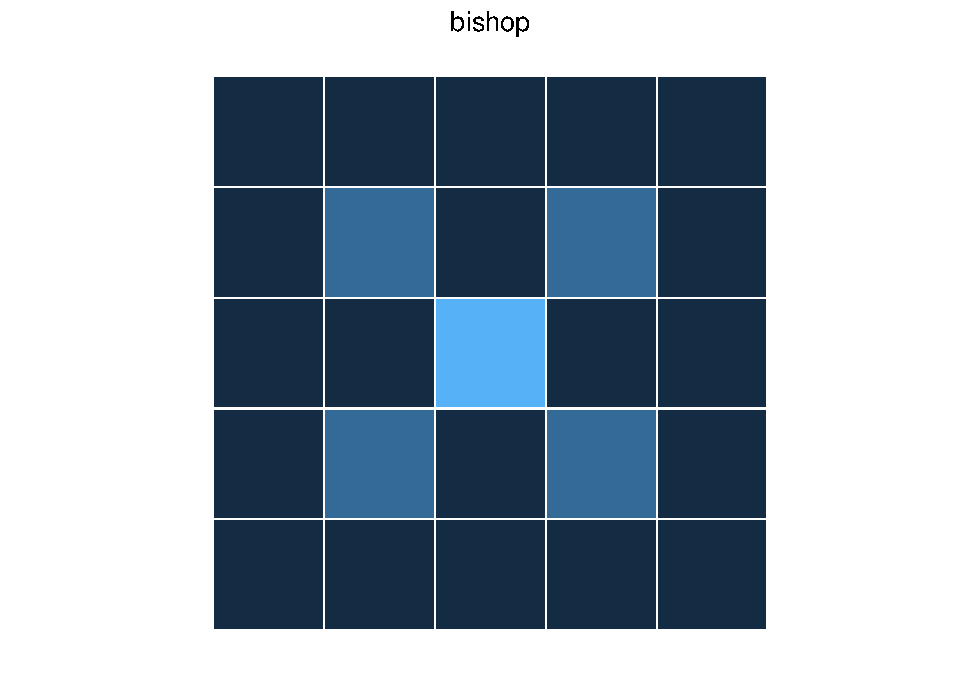
\includegraphics[width=0.25\linewidth]{midterm-project_files/figure-latex/unnamed-chunk-1-3}
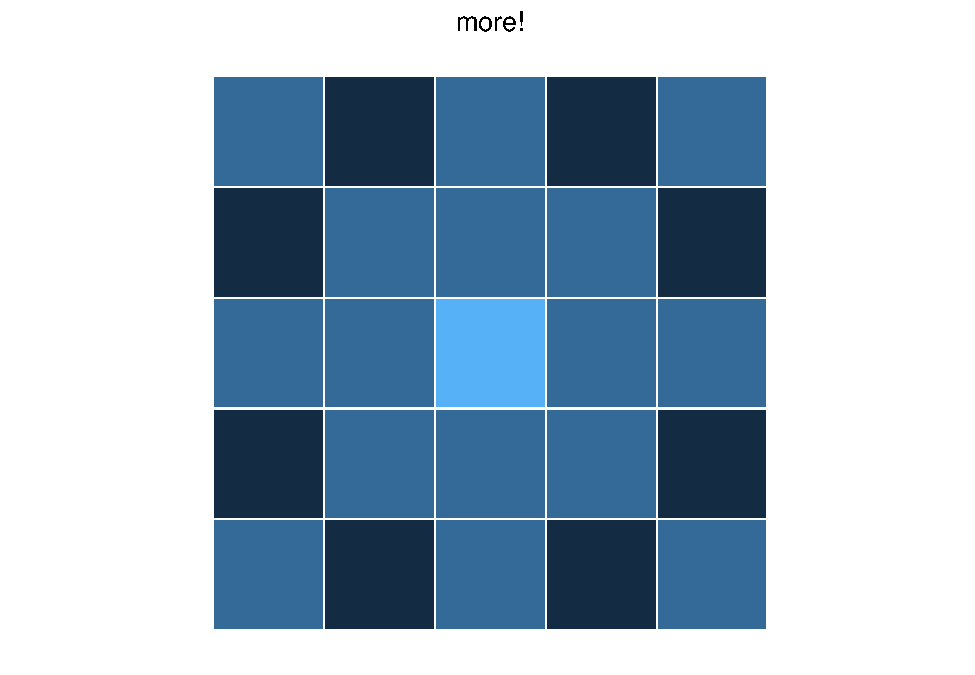
\includegraphics[width=0.25\linewidth]{midterm-project_files/figure-latex/unnamed-chunk-1-4}

Using these neighbor relationships we can create a
\texttt{weights\ matrix} based on understanding what the expected
relationships are between neighbors. The most simple example of this is
where the \(w_{ij}\) = 0 if the polygons are not neighbors and
\(w_{ij}\) = 1 if polygons are neighbors.

After we do our analysis we also need to check the residuals to ensure
we removed the spatial patterns.

\hypertarget{our-dataset}{%
\section{Our dataset}\label{our-dataset}}

The dataset we are using is published in \texttt{spData} package and
comes from: \emph{Anselin, Luc. 1988. Spatial econometrics: methods and
models. Dordrecht: Kluwer Academic, Table 12.1 p.~189.}

\begin{Shaded}
\begin{Highlighting}[]
\DocumentationTok{\#\# load dataset}
\NormalTok{columbus }\OtherTok{\textless{}{-}} \FunctionTok{vect}\NormalTok{(}\FunctionTok{system.file}\NormalTok{(}\StringTok{"shapes/columbus.shp"}\NormalTok{, }\AttributeTok{package=}\StringTok{"spData"}\NormalTok{)[}\DecValTok{1}\NormalTok{])}
\NormalTok{df.columbus }\OtherTok{\textless{}{-}} \FunctionTok{as.data.frame}\NormalTok{(columbus)}
\end{Highlighting}
\end{Shaded}

The county data is:

\begin{itemize}
\tightlist
\item
  \(\texttt{HOVAL}_i\) housing value (in \$1,000) of county
  \(i=1\dots49\)
\item
  \(\texttt{INC}_i\) household income (in \$1,000) of county
  \(i=1\dots49\)
\item
  \(\texttt{CRIME}_i\) residential burglaries and vehicle thefts per
  thousand households in the neighborhood of county \(i=1\dots49\)
\item
  \(\texttt{OPEN}_i\) open space in neighborhood of county
  \(i=1\dots49\)
\item
  \(\texttt{PLUMB}_i\) percentage housing units without plumbing of
  county \(i=1\dots49\)
\item
  \(\texttt{CP}_i\) core-periphery is an indicator variable
  \(I_{CP}(i)= \begin{cases}1 & \text { if county } i \text { is in the core } \\ 0 & \text { otherwise }\end{cases}\)
\end{itemize}

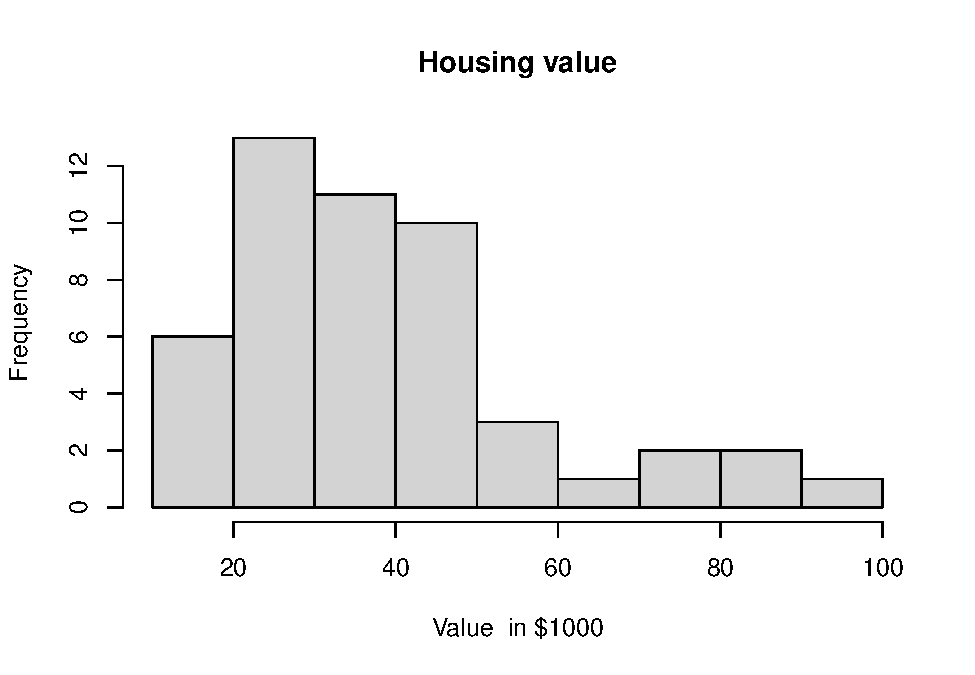
\includegraphics[width=0.5\linewidth]{midterm-project_files/figure-latex/unnamed-chunk-3-1}
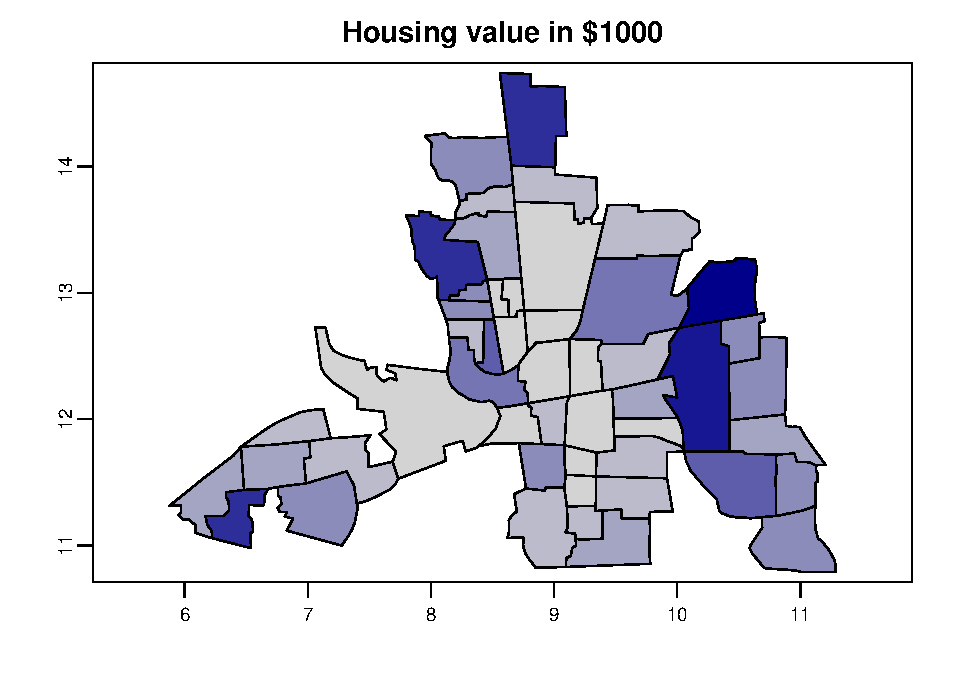
\includegraphics[width=0.5\linewidth]{midterm-project_files/figure-latex/unnamed-chunk-3-2}
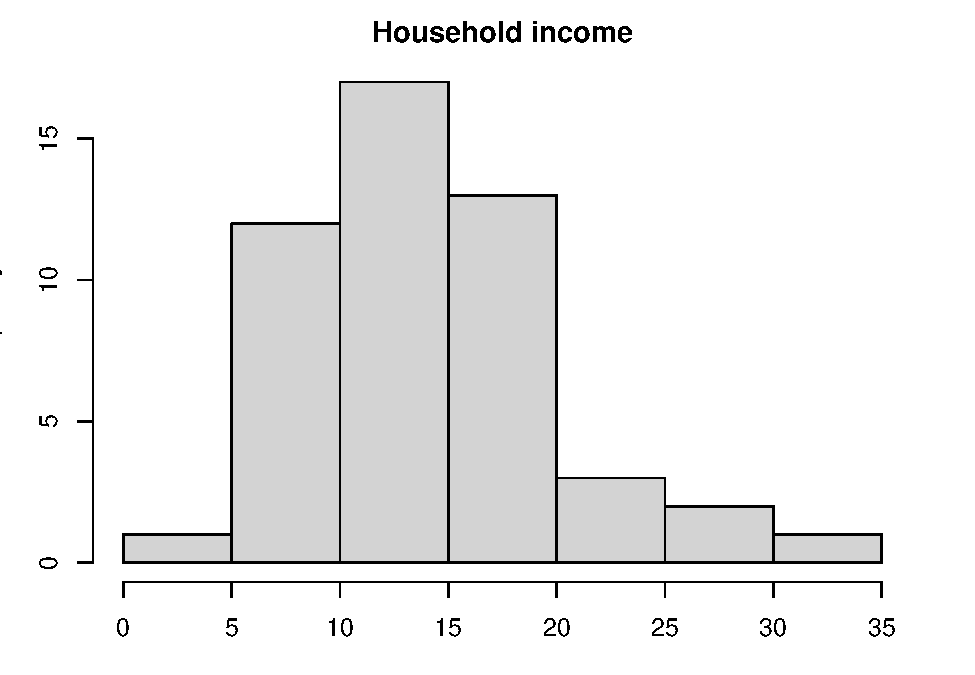
\includegraphics[width=0.5\linewidth]{midterm-project_files/figure-latex/unnamed-chunk-3-3}
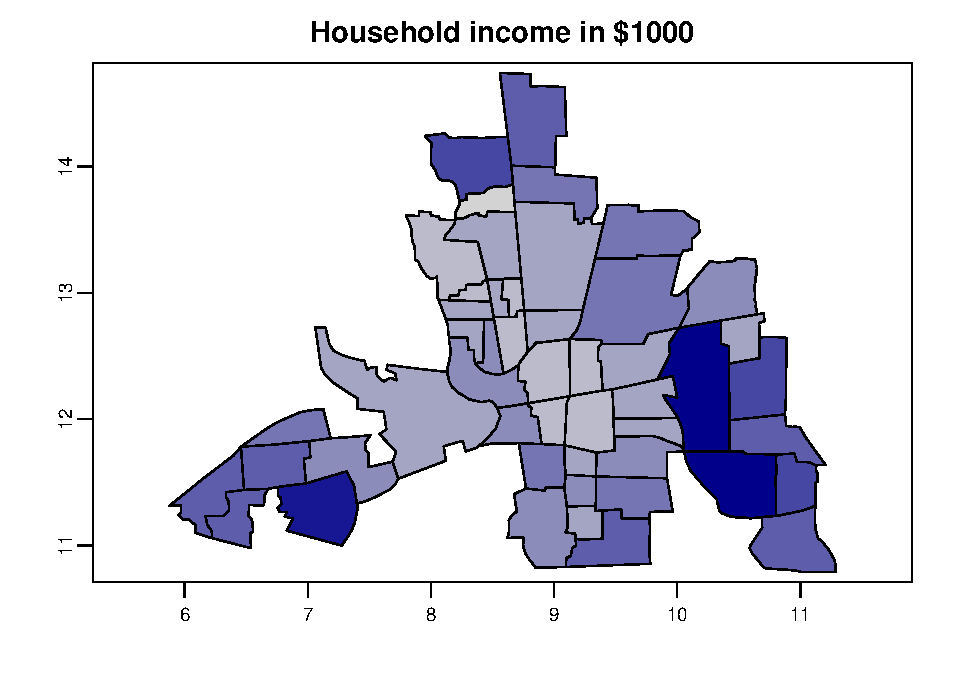
\includegraphics[width=0.5\linewidth]{midterm-project_files/figure-latex/unnamed-chunk-3-4}
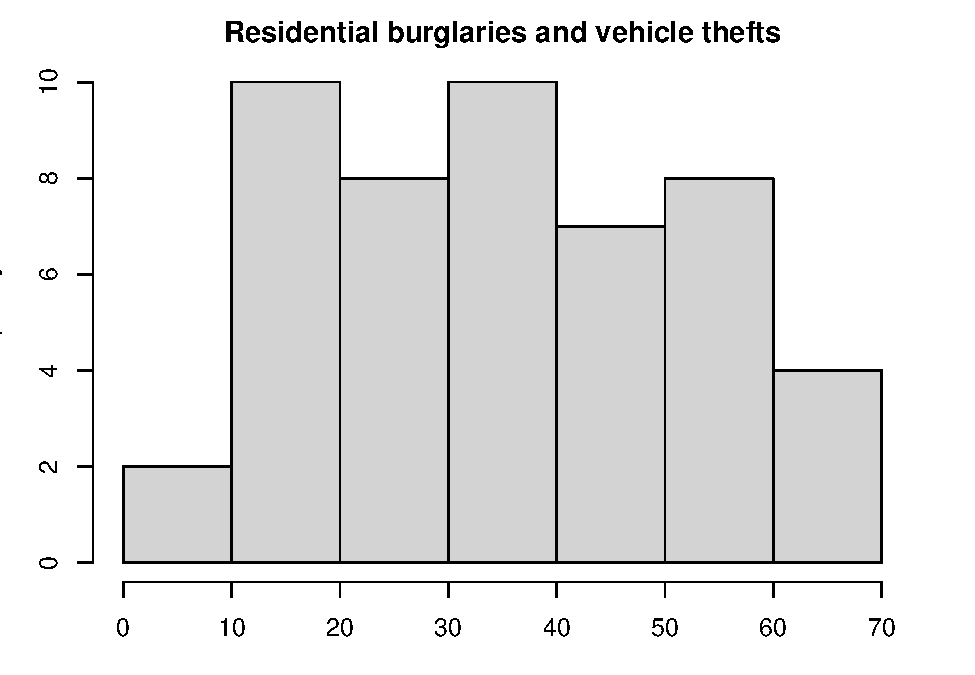
\includegraphics[width=0.5\linewidth]{midterm-project_files/figure-latex/unnamed-chunk-3-5}
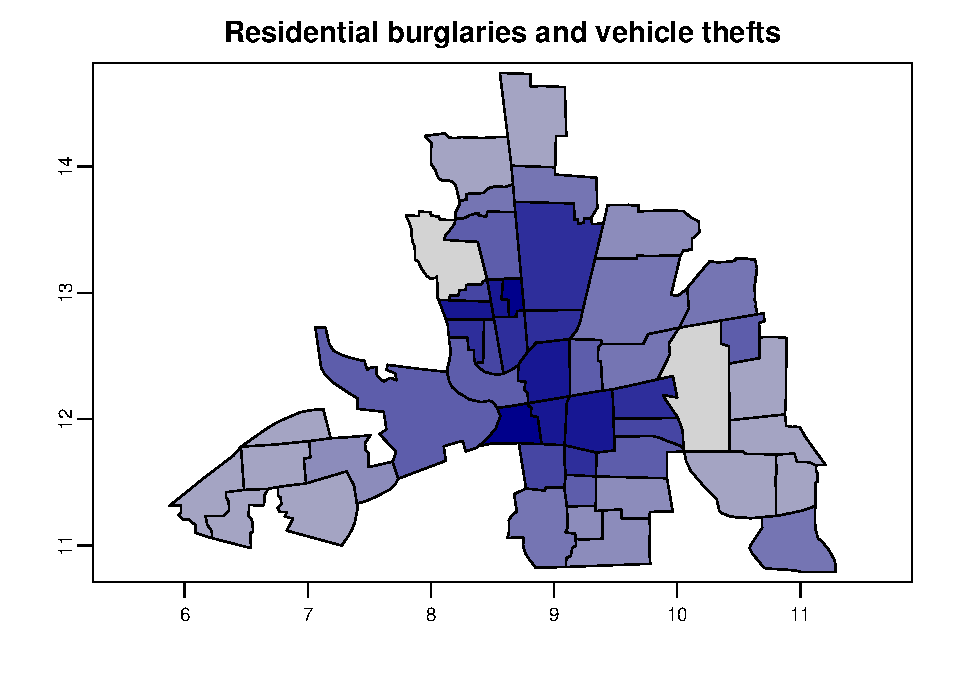
\includegraphics[width=0.5\linewidth]{midterm-project_files/figure-latex/unnamed-chunk-3-6}
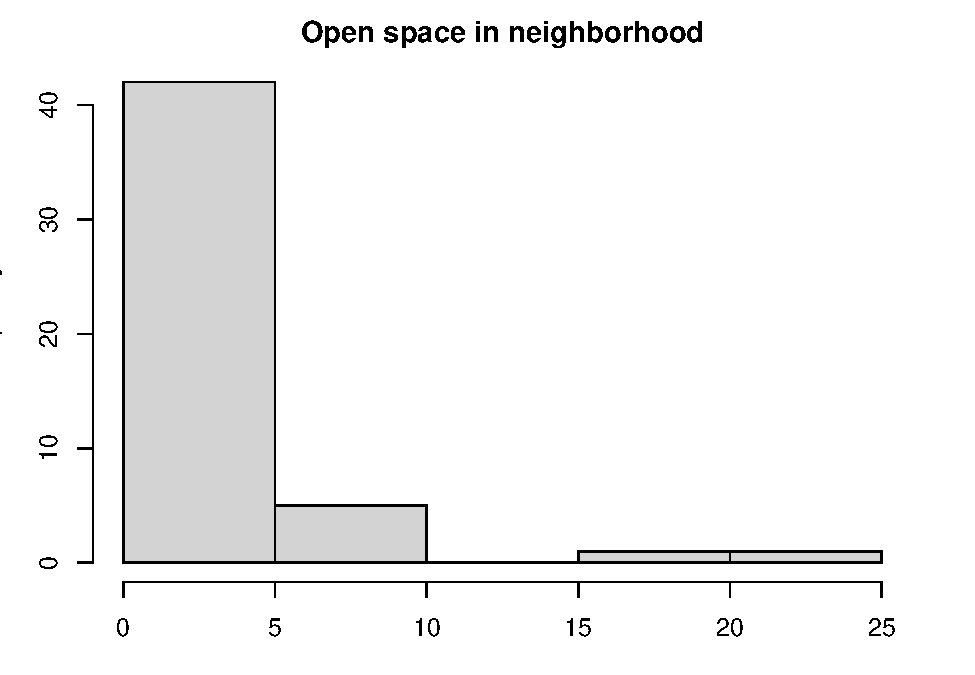
\includegraphics[width=0.5\linewidth]{midterm-project_files/figure-latex/unnamed-chunk-3-7}
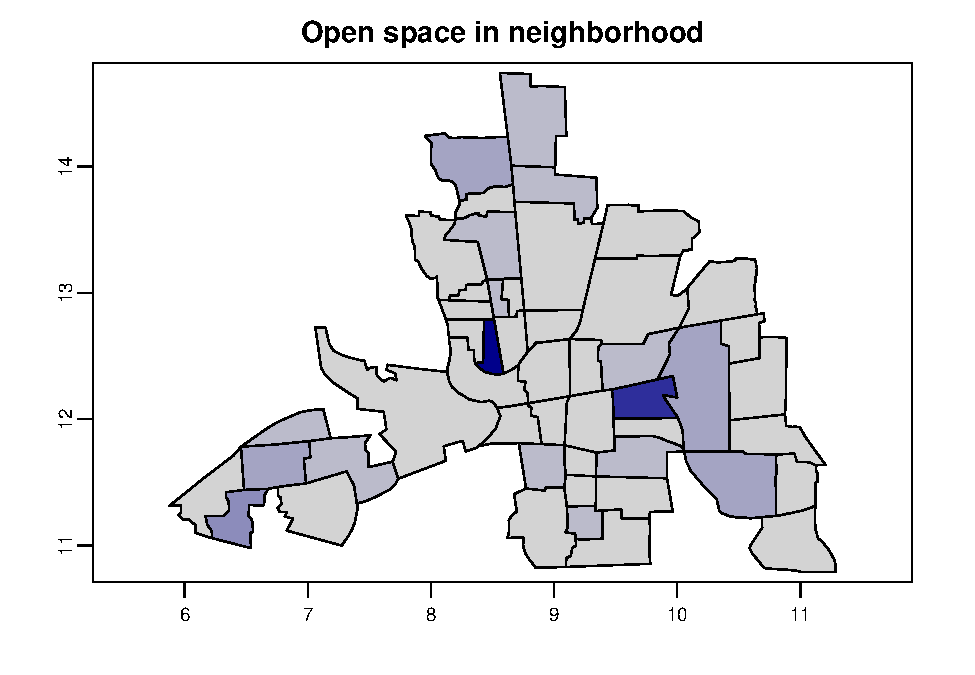
\includegraphics[width=0.5\linewidth]{midterm-project_files/figure-latex/unnamed-chunk-3-8}
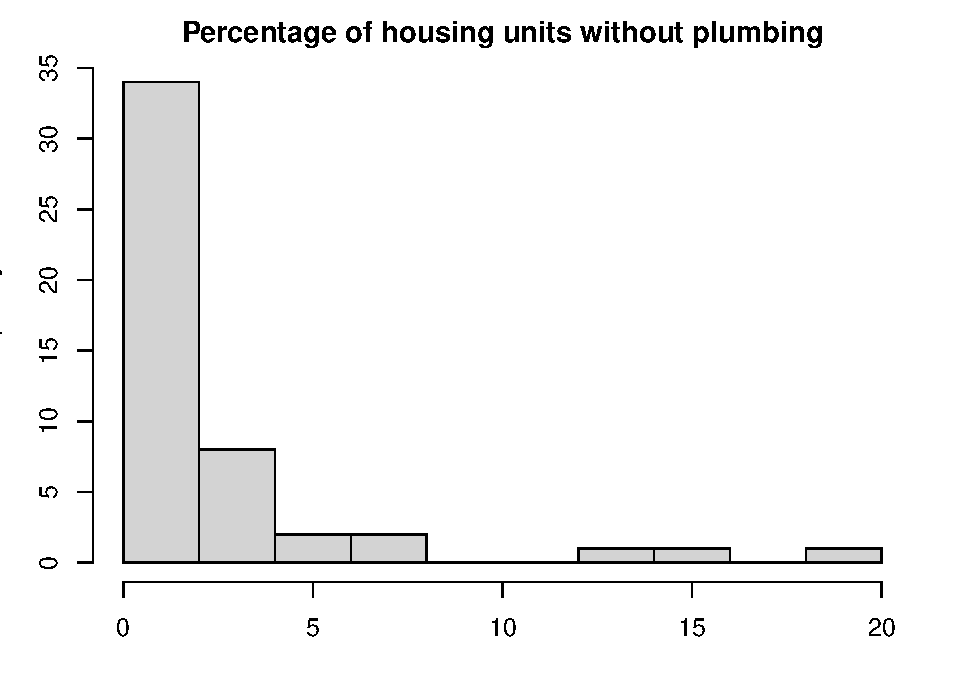
\includegraphics[width=0.5\linewidth]{midterm-project_files/figure-latex/unnamed-chunk-3-9}
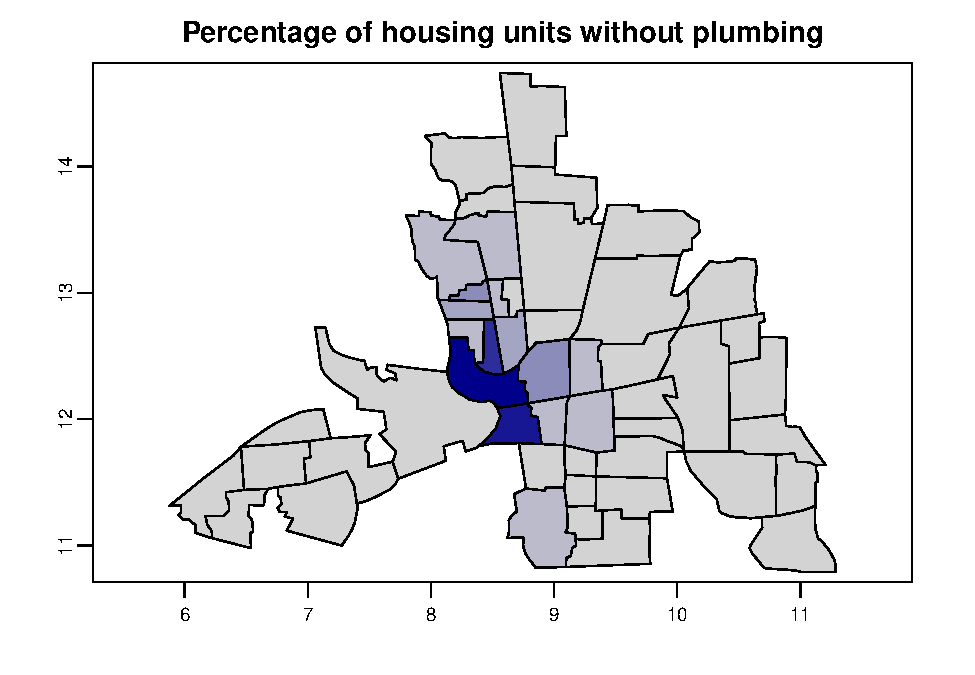
\includegraphics[width=0.5\linewidth]{midterm-project_files/figure-latex/unnamed-chunk-3-10}
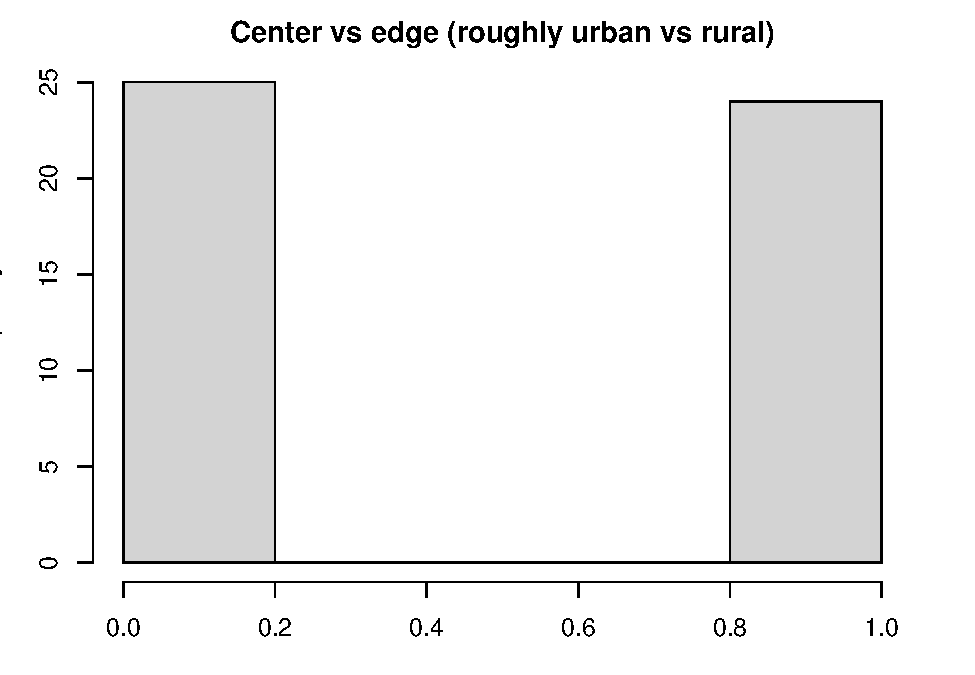
\includegraphics[width=0.5\linewidth]{midterm-project_files/figure-latex/unnamed-chunk-3-11}
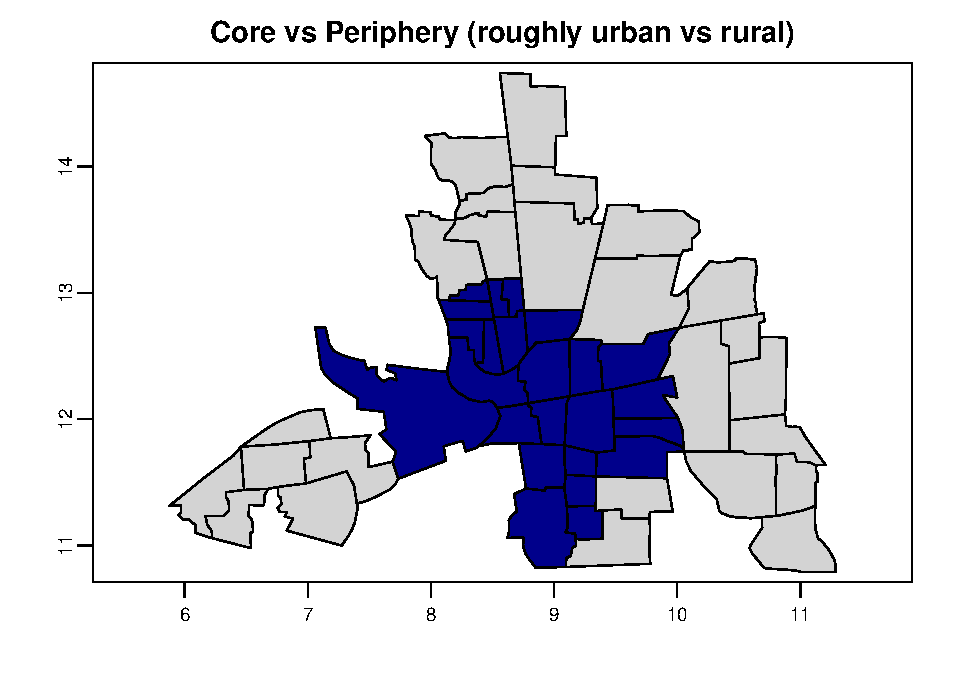
\includegraphics[width=0.5\linewidth]{midterm-project_files/figure-latex/unnamed-chunk-3-12}

Because we plan to use housing value as our response variable, a
logarithm transformation is applied to fix the skewness of the
distribution for the variable housing value.

\begin{Shaded}
\begin{Highlighting}[]
\CommentTok{\# Make histogram}
\FunctionTok{hist}\NormalTok{(}\FunctionTok{log}\NormalTok{(df.columbus}\SpecialCharTok{$}\NormalTok{HOVAL), }
     \AttributeTok{main =} \StringTok{"Housing value"}\NormalTok{, }
     \AttributeTok{xlab =} \StringTok{"Value  in $1000 (log)"}\NormalTok{)}
\end{Highlighting}
\end{Shaded}

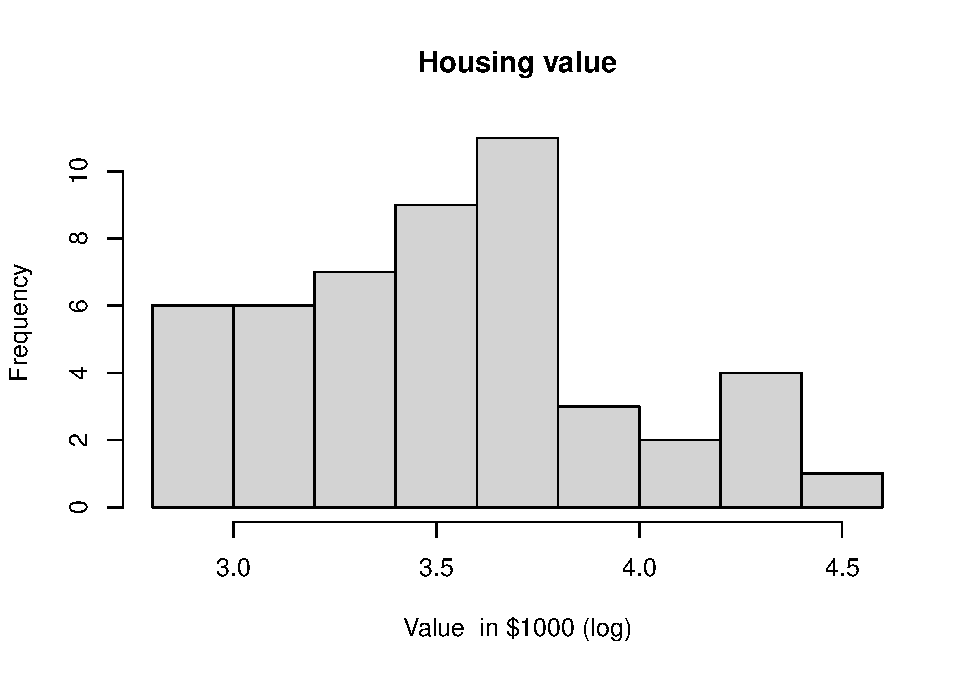
\includegraphics{midterm-project_files/figure-latex/unnamed-chunk-4-1.pdf}

\hypertarget{exploratory-data-analysis}{%
\section{Exploratory Data Analysis}\label{exploratory-data-analysis}}

\hypertarget{measures-of-spatial-association}{%
\subsection{Measures of spatial
association}\label{measures-of-spatial-association}}

\hypertarget{neighbors}{%
\subsubsection{Neighbors}\label{neighbors}}

There are a many options when making the adjacency matrix as outlined
above, but for our purposes we are saying that any counties touching
each other are neighbors (1s) and any that aren't are not (0s). This is
the neighbor schema shown in the queen/touches plot above.

Figure out what the neighbors are, we must decide a few rule. Here we
are considering all counties \(i=1\dots49\) and \(j=1\dots49\) that
touch each other to be neighbors and that the relationship is
symmetrical (i.e.~\(w_{ij}\) = \(w_{ji}\))

\begin{Shaded}
\begin{Highlighting}[]
\NormalTok{xy }\OtherTok{\textless{}{-}}\NormalTok{ terra}\SpecialCharTok{::}\FunctionTok{centroids}\NormalTok{(columbus)}
\NormalTok{neighbors }\OtherTok{\textless{}{-}} \FunctionTok{adjacent}\NormalTok{(columbus, }\AttributeTok{type =} \StringTok{"touches"}\NormalTok{, }\AttributeTok{symmetrical=}\ConstantTok{TRUE}\NormalTok{)}
\FunctionTok{colnames}\NormalTok{(neighbors) }\OtherTok{\textless{}{-}} \FunctionTok{c}\NormalTok{(}\StringTok{"i"}\NormalTok{, }\StringTok{"j"}\NormalTok{)}
\CommentTok{\# head(neighbors)}
\FunctionTok{plot}\NormalTok{(columbus, }\AttributeTok{col=}\StringTok{\textquotesingle{}lightgray\textquotesingle{}}\NormalTok{, }\AttributeTok{border=}\StringTok{\textquotesingle{}black\textquotesingle{}}\NormalTok{, }\AttributeTok{lwd=}\DecValTok{1}\NormalTok{)}
\NormalTok{p1 }\OtherTok{\textless{}{-}}\NormalTok{ xy[neighbors[,}\DecValTok{1}\NormalTok{], ]}
\NormalTok{p2 }\OtherTok{\textless{}{-}}\NormalTok{ xy[neighbors[,}\DecValTok{2}\NormalTok{], ]}
\FunctionTok{lines}\NormalTok{(p1, p2, }\AttributeTok{col=}\StringTok{\textquotesingle{}red\textquotesingle{}}\NormalTok{, }\AttributeTok{lwd=}\DecValTok{2}\NormalTok{)}
\end{Highlighting}
\end{Shaded}

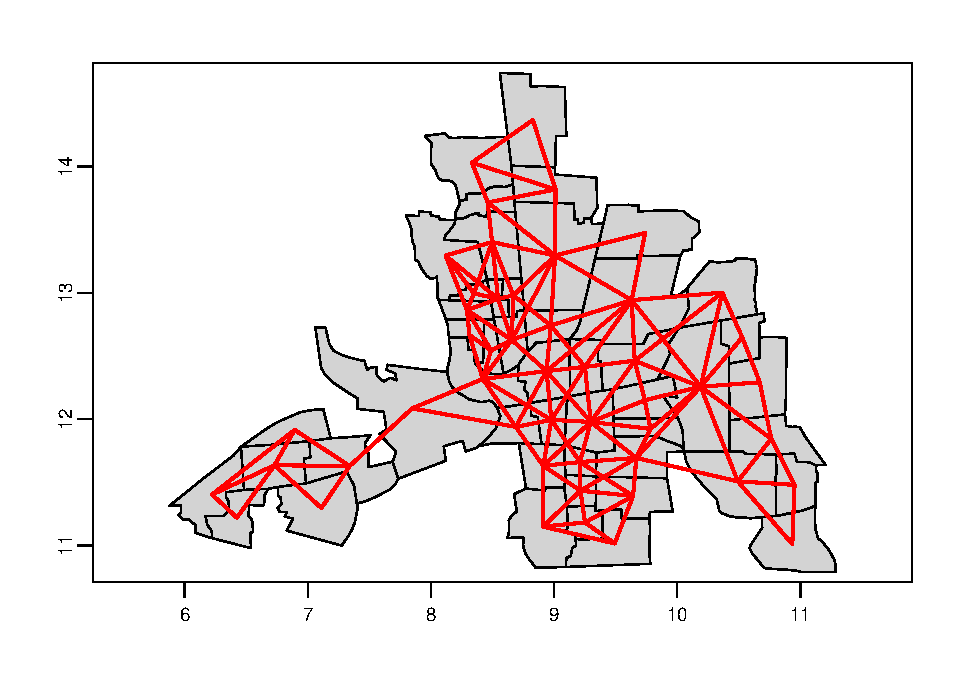
\includegraphics{midterm-project_files/figure-latex/unnamed-chunk-5-1.pdf}

In the weight matrix any counties touching each other are neighbors and
assigned a weight of 1 (\(w_{ij}\) = 1) and any that are not touching
each other are assigned a weight of 0 (\(w_{ij}\) = 0).

Here is what part of the adjacency matrix looks like:

\begin{Shaded}
\begin{Highlighting}[]
\FunctionTok{adjacent}\NormalTok{(columbus, }\StringTok{"touches"}\NormalTok{, }\AttributeTok{pairs =} \ConstantTok{FALSE}\NormalTok{)[}\DecValTok{1}\SpecialCharTok{:}\DecValTok{10}\NormalTok{,}\DecValTok{1}\SpecialCharTok{:}\DecValTok{10}\NormalTok{]}
\end{Highlighting}
\end{Shaded}

\begin{verbatim}
##    1 2 3 4 5 6 7 8 9 10
## 1  0 1 1 0 0 0 0 0 0  0
## 2  1 0 1 1 0 0 0 0 0  0
## 3  1 1 0 1 1 0 0 0 0  0
## 4  0 1 1 0 1 0 0 1 0  0
## 5  0 0 1 1 0 1 0 1 1  0
## 6  0 0 0 0 1 0 0 0 1  0
## 7  0 0 0 0 0 0 0 1 0  0
## 8  0 0 0 1 1 0 1 0 0  0
## 9  0 0 0 0 1 1 0 0 0  1
## 10 0 0 0 0 0 0 0 0 1  0
\end{verbatim}

From that we can understand that county\(_{i=1}\) is touching
counties\(_{j = 2, 3}\) and not touching counties\(_{j=4\dots10}\),
because the weights of \(w_{1,2}, w_{1,3}\) = 1 and \(w_{1,4\dots10}\) =
0.

\hypertarget{morans-i}{%
\subsubsection{Moran's I}\label{morans-i}}

Moran's \(I\) is a global measure of spatial autocorrelation with values
ranging -1 to 1. Here we are using a neighbor's matrix for any counties
that are touching each other (\(w_{ij}\)). \(n\) is the number of
neighborhoods in Columbus, OH which are indexed by \(i\) and \(j\) (is
polygon \(i\) a neighbor with \(j\). \(\overline{y}\) is the mean value
of the variable of interest and \(y_{1...n}\) is that value in each
polygon.

The assumptions for this test are (Bivand et al., 2013):

\begin{itemize}
\tightlist
\item
  ``the mean model of the data removes systematic spatial patterning
  from the data''\\
\item
  the observed spatial autocorrelation is not due to an underlying
  process in our model (i.e.~a parameter controlled for in the model)\\
\item
  the chosen weights matrix suits the underlying interactions between
  the polygons
\end{itemize}

The main limitation of this method is that the model variance can be
misspecified because it does not meet one of the assumptions above,
e.g.~the chosen weights matrix needs to suit the underlying interactions
between the polygons.

\[
I=\frac{n}{\sum_{i=1}^{n} \sum_{j=1}^{n} w_{ij}} \frac{\sum_{i=1}^{n} \sum_{j=1}^{n} w_{ij} (y_{i}-\overline{y}) (y_{j}-\overline{y})}{\sum_{i=1}^{n} (y_{i}-\overline{y})^{2}}
\] Using the \texttt{terra} package to test for spatial autocorrelation
of each variable, by county in Columbus, OH.

The adjacency matrix for all counties that touch each other (\(w_{ij}\)
above):

\begin{Shaded}
\begin{Highlighting}[]
\NormalTok{ww }\OtherTok{\textless{}{-}}  \FunctionTok{adjacent}\NormalTok{(columbus, }\StringTok{"touches"}\NormalTok{, }\AttributeTok{pairs=}\ConstantTok{FALSE}\NormalTok{)}
\end{Highlighting}
\end{Shaded}

Roughly the expected value for Moran's I is \(E(I)=\frac{-1}{n-1}\)

\begin{Shaded}
\begin{Highlighting}[]
\NormalTok{(}\AttributeTok{ev =} \SpecialCharTok{{-}}\DecValTok{1}\SpecialCharTok{/}\NormalTok{(}\FunctionTok{nrow}\NormalTok{(columbus)}\SpecialCharTok{{-}}\DecValTok{1}\NormalTok{))}
\end{Highlighting}
\end{Shaded}

\begin{verbatim}
## [1] -0.02083333
\end{verbatim}

The null hypothesis \(H_0\) is that the values are distributed following
a random process or with negative spatial autocorrelation (I \textless=
-0.021), and the alternative hypothesis \(H_1\) is that the values are
distributed with positive spatial autocorrelation (I \textgreater{}
-0.021). We are using a significance level of \(\alpha = 0.05\).
Negative spatial autocorrelation is a phenomena that generally occurs in
random dataset. Positive spatial autocorrelation indicates neighbors are
more similar to each other than non-neighbors. The p-value is calculated
using a Monte Carlo simulation, from which we derive a density plot of
the I values from each permutation and calculate the number of times our
simulated I value is greater than or equal to the observed value out of
all the trials. A monte carlo simulation is the best method for this
because it is robust to irregularly shaped polygons.

\hypertarget{house-value}{%
\paragraph{House value}\label{house-value}}

\begin{Shaded}
\begin{Highlighting}[]
\DocumentationTok{\#\# Moran\textquotesingle{}s I}
\NormalTok{(ac }\OtherTok{\textless{}{-}} \FunctionTok{autocor}\NormalTok{(columbus}\SpecialCharTok{$}\NormalTok{HOVAL, ww, }\StringTok{"moran"}\NormalTok{))}
\end{Highlighting}
\end{Shaded}

\begin{verbatim}
## [1] 0.2213441
\end{verbatim}

\begin{Shaded}
\begin{Highlighting}[]
\DocumentationTok{\#\# Monte Carlo sim to test for significance }
\NormalTok{m }\OtherTok{\textless{}{-}} \FunctionTok{sapply}\NormalTok{(}\DecValTok{1}\SpecialCharTok{:}\DecValTok{99}\NormalTok{, }\ControlFlowTok{function}\NormalTok{(i) \{}
    \FunctionTok{autocor}\NormalTok{(}\FunctionTok{sample}\NormalTok{(columbus}\SpecialCharTok{$}\NormalTok{HOVAL), ww, }\StringTok{"moran"}\NormalTok{)}
\NormalTok{\})}
\FunctionTok{plot}\NormalTok{(}\FunctionTok{density}\NormalTok{(m), }\AttributeTok{main =} \ConstantTok{NA}\NormalTok{); }\FunctionTok{abline}\NormalTok{(}\AttributeTok{v=}\NormalTok{ac, }\AttributeTok{col =} \StringTok{"red"}\NormalTok{, }\AttributeTok{lwd =} \DecValTok{2}\NormalTok{) }\CommentTok{\#distribution of values of I using subsets of dataset}
\end{Highlighting}
\end{Shaded}

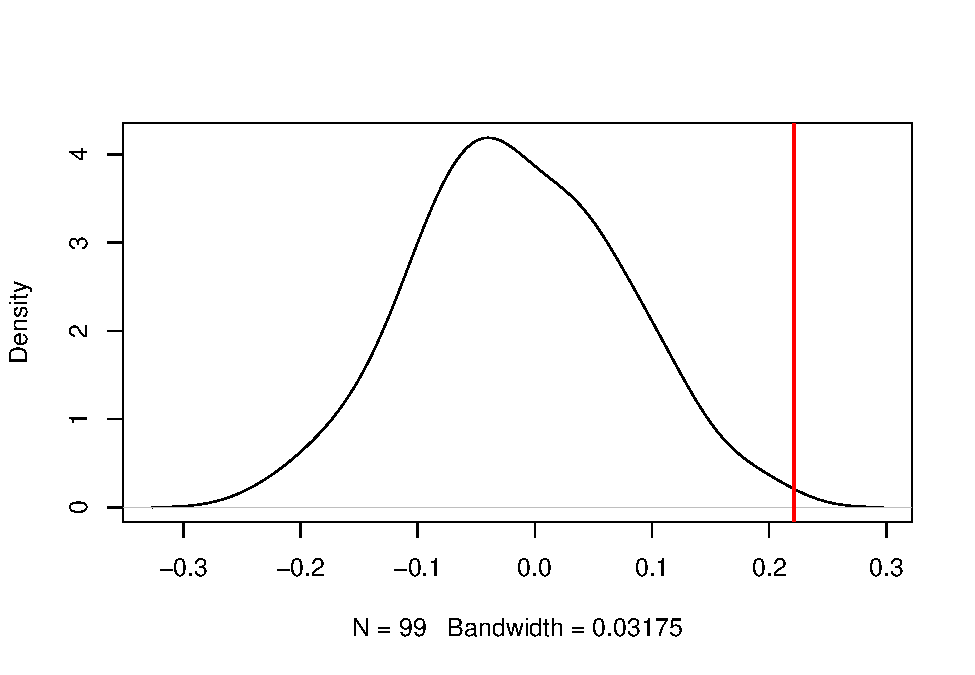
\includegraphics[width=0.5\linewidth]{midterm-project_files/figure-latex/unnamed-chunk-9-1}

\begin{Shaded}
\begin{Highlighting}[]
\DocumentationTok{\#\# p{-}value}
\FunctionTok{sum}\NormalTok{(m }\SpecialCharTok{\textgreater{}=}\NormalTok{ ac) }\SpecialCharTok{/} \DecValTok{100} \CommentTok{\# number of times I of subset is \textgreater{}= to I of entire dataset / number of trials}
\end{Highlighting}
\end{Shaded}

\begin{verbatim}
## [1] 0
\end{verbatim}

So there is significant (Moran's I = 0.2213441, p \textless{} 0.05)
spatial autocorrelation in house value, meaning the average value of
houses in neighboring neighborhoods are different from the average value
of all neighborhoods.

\hypertarget{household-income}{%
\paragraph{Household income}\label{household-income}}

\begin{Shaded}
\begin{Highlighting}[]
\DocumentationTok{\#\# Moran\textquotesingle{}s I}
\NormalTok{(ac }\OtherTok{\textless{}{-}} \FunctionTok{autocor}\NormalTok{(columbus}\SpecialCharTok{$}\NormalTok{INC, ww, }\StringTok{"moran"}\NormalTok{))}
\end{Highlighting}
\end{Shaded}

\begin{verbatim}
## [1] 0.412344
\end{verbatim}

\begin{Shaded}
\begin{Highlighting}[]
\DocumentationTok{\#\# sim}
\NormalTok{m }\OtherTok{\textless{}{-}} \FunctionTok{sapply}\NormalTok{(}\DecValTok{1}\SpecialCharTok{:}\DecValTok{99}\NormalTok{, }\ControlFlowTok{function}\NormalTok{(i) \{}
    \FunctionTok{autocor}\NormalTok{(}\FunctionTok{sample}\NormalTok{(columbus}\SpecialCharTok{$}\NormalTok{INC), ww, }\StringTok{"moran"}\NormalTok{)}
\NormalTok{\})}


\DocumentationTok{\#\# p{-}value}
\FunctionTok{sum}\NormalTok{(m }\SpecialCharTok{\textgreater{}=}\NormalTok{ ac) }\SpecialCharTok{/} \DecValTok{100}
\end{Highlighting}
\end{Shaded}

\begin{verbatim}
## [1] 0
\end{verbatim}

There is significant positive (Moran's I = 0.412344, p \textless{} 0.05)
Spatial autocorrelation in household income.

\hypertarget{crime}{%
\paragraph{Crime}\label{crime}}

\begin{Shaded}
\begin{Highlighting}[]
\DocumentationTok{\#\# Moran\textquotesingle{}s I}
\NormalTok{(ac }\OtherTok{\textless{}{-}} \FunctionTok{autocor}\NormalTok{(columbus}\SpecialCharTok{$}\NormalTok{CRIME, ww, }\StringTok{"moran"}\NormalTok{))}
\end{Highlighting}
\end{Shaded}

\begin{verbatim}
## [1] 0.5154614
\end{verbatim}

\begin{Shaded}
\begin{Highlighting}[]
\DocumentationTok{\#\#sim}
\NormalTok{m }\OtherTok{\textless{}{-}} \FunctionTok{sapply}\NormalTok{(}\DecValTok{1}\SpecialCharTok{:}\DecValTok{99}\NormalTok{, }\ControlFlowTok{function}\NormalTok{(i) \{}
    \FunctionTok{autocor}\NormalTok{(}\FunctionTok{sample}\NormalTok{(columbus}\SpecialCharTok{$}\NormalTok{CRIME), ww, }\StringTok{"moran"}\NormalTok{)}
\NormalTok{\})}

\DocumentationTok{\#\# p{-}value}
\FunctionTok{sum}\NormalTok{(m }\SpecialCharTok{\textgreater{}=}\NormalTok{ ac) }\SpecialCharTok{/} \DecValTok{100}
\end{Highlighting}
\end{Shaded}

\begin{verbatim}
## [1] 0
\end{verbatim}

So again we see significant spatial autocorrelation (Moran's I =
0.5154614, p \textless{} 0.05).

\hypertarget{open-space}{%
\paragraph{Open space}\label{open-space}}

\begin{Shaded}
\begin{Highlighting}[]
\DocumentationTok{\#\# Moran\textquotesingle{}s I}
\NormalTok{(ac }\OtherTok{\textless{}{-}} \FunctionTok{autocor}\NormalTok{(columbus}\SpecialCharTok{$}\NormalTok{OPEN, ww, }\StringTok{"moran"}\NormalTok{))}
\end{Highlighting}
\end{Shaded}

\begin{verbatim}
## [1] -0.03669849
\end{verbatim}

\begin{Shaded}
\begin{Highlighting}[]
\DocumentationTok{\#\# sim}
\NormalTok{m }\OtherTok{\textless{}{-}} \FunctionTok{sapply}\NormalTok{(}\DecValTok{1}\SpecialCharTok{:}\DecValTok{99}\NormalTok{, }\ControlFlowTok{function}\NormalTok{(i) \{}
    \FunctionTok{autocor}\NormalTok{(}\FunctionTok{sample}\NormalTok{(columbus}\SpecialCharTok{$}\NormalTok{HOVAL), ww, }\StringTok{"moran"}\NormalTok{)}
\NormalTok{\})}

\DocumentationTok{\#\# p{-}value}
\FunctionTok{sum}\NormalTok{(m }\SpecialCharTok{\textgreater{}=}\NormalTok{ ac) }\SpecialCharTok{/} \DecValTok{100}
\end{Highlighting}
\end{Shaded}

\begin{verbatim}
## [1] 0.58
\end{verbatim}

There is not spatial autocorrelation with open space (Moran's I =
-0.0366985; p-value \textgreater{} 0.05)

\hypertarget{plumbing}{%
\paragraph{Plumbing}\label{plumbing}}

\begin{Shaded}
\begin{Highlighting}[]
\DocumentationTok{\#\# Moran\textquotesingle{}s I}
\NormalTok{(ac }\OtherTok{\textless{}{-}} \FunctionTok{autocor}\NormalTok{(columbus}\SpecialCharTok{$}\NormalTok{PLUMB, ww, }\StringTok{"moran"}\NormalTok{))}
\end{Highlighting}
\end{Shaded}

\begin{verbatim}
## [1] 0.4550575
\end{verbatim}

\begin{Shaded}
\begin{Highlighting}[]
\DocumentationTok{\#\# sim}
\NormalTok{m }\OtherTok{\textless{}{-}} \FunctionTok{sapply}\NormalTok{(}\DecValTok{1}\SpecialCharTok{:}\DecValTok{99}\NormalTok{, }\ControlFlowTok{function}\NormalTok{(i) \{}
    \FunctionTok{autocor}\NormalTok{(}\FunctionTok{sample}\NormalTok{(columbus}\SpecialCharTok{$}\NormalTok{HOVAL), ww, }\StringTok{"moran"}\NormalTok{)}
\NormalTok{\})}

\DocumentationTok{\#\# p{-}value}
\FunctionTok{sum}\NormalTok{(m }\SpecialCharTok{\textgreater{}=}\NormalTok{ ac) }\SpecialCharTok{/} \DecValTok{100}
\end{Highlighting}
\end{Shaded}

\begin{verbatim}
## [1] 0
\end{verbatim}

There is significant spatial autocorrelation with plumbing (Moran's I =
0.4550575, p \textless{} 0.05).

\hypertarget{gearys-c}{%
\subsubsection{Geary's C}\label{gearys-c}}

Geary's \(C\) is a measure of global measure of spatial autocorrelation
that is more sensitive to local correlations. It is roughly inversely
related to Moran's I. The values ranging 0 to greater than 1, with
values 0-1 representing positive spatial autocorrelation and values
\textgreater{} 1 representing negative spatial autocorrelation.

The neighbor's matrix (\(w_{ij}\)) is the same what was used for Moran's
I. \(N\) is the number of spatial units indexed by i and j; \(y\) is the
variable of interest; \(\bar{y}\) is the mean of \(y\); \(w_{ij}\) is a
matrix of spatial weights with zeroes on the diagonal (i.e.,
\(w_{ii}=0\)); and \(W\) is the sum of all \(w_{ij}\).
\(\sum_{i \neq j} w_{i j}\) is the sum of that weight matrix with the
diagonal equal to 0.\\
\[
C=\frac{(n-1) \sum_{i} \sum_{j} w_{i j}\left(y_{i}-y_{j}\right)^{2}}{2\left(\sum_{i \neq j} w_{i j}\right) \sum_{i}\left(y_{i}-\bar{y}\right)^{2}}
\]

The null hypothesis here is that the values are distributed following a
random process or have negative spatial autocorrelation (C \textgreater=
1), and the alternative hypothesis is that the values are distributed
with positive spatial autocorrelation (C \textless{} 1). The p-value is
calculated using a Monte Carlo simulation, from which we derive a
density plot of the C values from each permutation and calculate the
number of times our simulated C value is greater than or equal to the
observed value out of all the trials. A monte carlo simulation is the
best method for this because it is robust to irregularly shaped
polygons.

\hypertarget{house-value-1}{%
\paragraph{House Value}\label{house-value-1}}

\begin{Shaded}
\begin{Highlighting}[]
\NormalTok{(gearyc }\OtherTok{\textless{}{-}} \FunctionTok{autocor}\NormalTok{(columbus}\SpecialCharTok{$}\NormalTok{HOVAL, ww, }\StringTok{"geary"}\NormalTok{))}
\end{Highlighting}
\end{Shaded}

\begin{verbatim}
## [1] 0.7889937
\end{verbatim}

\begin{Shaded}
\begin{Highlighting}[]
\DocumentationTok{\#\# Monte Carlo sim to test for significance }
\NormalTok{m }\OtherTok{\textless{}{-}} \FunctionTok{sapply}\NormalTok{(}\DecValTok{1}\SpecialCharTok{:}\DecValTok{99}\NormalTok{, }\ControlFlowTok{function}\NormalTok{(i) \{}
    \FunctionTok{autocor}\NormalTok{(}\FunctionTok{sample}\NormalTok{(columbus}\SpecialCharTok{$}\NormalTok{HOVAL), ww, }\StringTok{"geary"}\NormalTok{)}
\NormalTok{\})}
\FunctionTok{plot}\NormalTok{(}\FunctionTok{density}\NormalTok{(m), }\AttributeTok{main =} \ConstantTok{NA}\NormalTok{); }\FunctionTok{abline}\NormalTok{(}\AttributeTok{v=}\NormalTok{gearyc, }\AttributeTok{col =} \StringTok{"red"}\NormalTok{, }\AttributeTok{lwd =} \DecValTok{2}\NormalTok{)}
\end{Highlighting}
\end{Shaded}

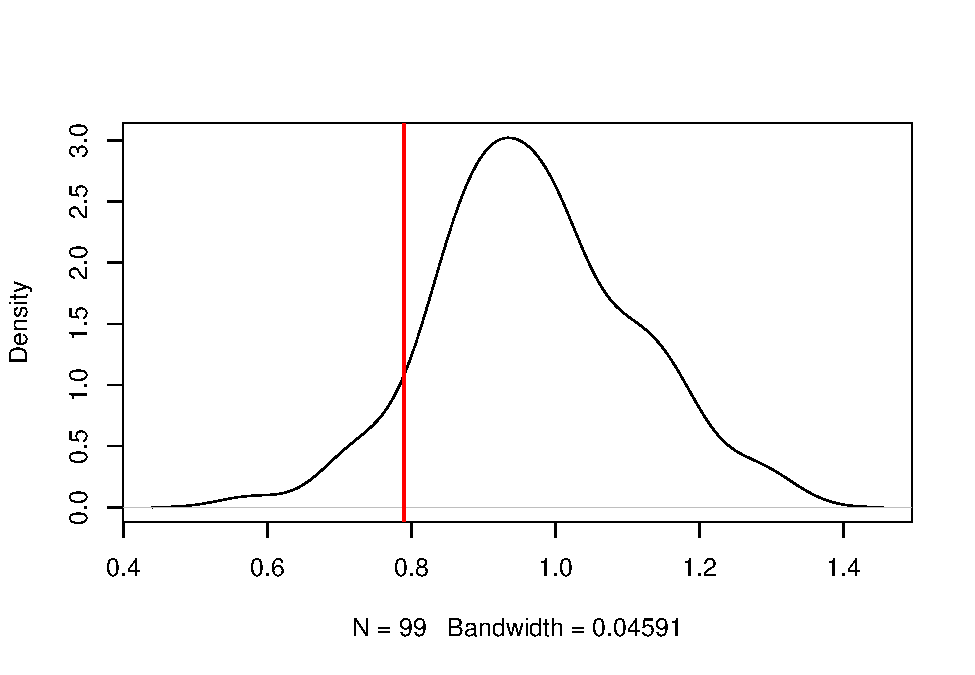
\includegraphics[width=0.5\linewidth]{midterm-project_files/figure-latex/unnamed-chunk-19-1}

\begin{Shaded}
\begin{Highlighting}[]
\DocumentationTok{\#\# p{-}value}
\FunctionTok{sum}\NormalTok{(m }\SpecialCharTok{\textless{}=}\NormalTok{ gearyc) }\SpecialCharTok{/} \DecValTok{100}
\end{Highlighting}
\end{Shaded}

\begin{verbatim}
## [1] 0.07
\end{verbatim}

No significant spatial autocorrelation (geary's c = 0.7889937, p
\textgreater{} 0.05).

\hypertarget{household-income-1}{%
\paragraph{Household Income}\label{household-income-1}}

\begin{Shaded}
\begin{Highlighting}[]
\NormalTok{(gearyc }\OtherTok{\textless{}{-}} \FunctionTok{autocor}\NormalTok{(columbus}\SpecialCharTok{$}\NormalTok{INC, ww, }\StringTok{"geary"}\NormalTok{))}
\end{Highlighting}
\end{Shaded}

\begin{verbatim}
## [1] 0.7137603
\end{verbatim}

\begin{Shaded}
\begin{Highlighting}[]
\DocumentationTok{\#\# Monte Carlo sim to test for significance }
\NormalTok{m }\OtherTok{\textless{}{-}} \FunctionTok{sapply}\NormalTok{(}\DecValTok{1}\SpecialCharTok{:}\DecValTok{99}\NormalTok{, }\ControlFlowTok{function}\NormalTok{(i) \{}
    \FunctionTok{autocor}\NormalTok{(}\FunctionTok{sample}\NormalTok{(columbus}\SpecialCharTok{$}\NormalTok{INC), ww, }\StringTok{"geary"}\NormalTok{)}
\NormalTok{\})}

\DocumentationTok{\#\# p{-}value}
\FunctionTok{sum}\NormalTok{(m }\SpecialCharTok{\textless{}=}\NormalTok{ gearyc) }\SpecialCharTok{/} \DecValTok{100}
\end{Highlighting}
\end{Shaded}

\begin{verbatim}
## [1] 0
\end{verbatim}

Significant spatial autocorrelation (geary's c = 0.7137603, p
\textless{} 0.05).

\hypertarget{crime-1}{%
\paragraph{Crime}\label{crime-1}}

\begin{Shaded}
\begin{Highlighting}[]
\NormalTok{(gearyc }\OtherTok{\textless{}{-}} \FunctionTok{autocor}\NormalTok{(columbus}\SpecialCharTok{$}\NormalTok{CRIME, ww, }\StringTok{"geary"}\NormalTok{))}
\end{Highlighting}
\end{Shaded}

\begin{verbatim}
## [1] 0.5916113
\end{verbatim}

\begin{Shaded}
\begin{Highlighting}[]
\DocumentationTok{\#\# Monte Carlo sim to test for significance }
\NormalTok{m }\OtherTok{\textless{}{-}} \FunctionTok{sapply}\NormalTok{(}\DecValTok{1}\SpecialCharTok{:}\DecValTok{99}\NormalTok{, }\ControlFlowTok{function}\NormalTok{(i) \{}
    \FunctionTok{autocor}\NormalTok{(}\FunctionTok{sample}\NormalTok{(columbus}\SpecialCharTok{$}\NormalTok{CRIME), ww, }\StringTok{"geary"}\NormalTok{)}
\NormalTok{\})}

\DocumentationTok{\#\# p{-}value}
\FunctionTok{sum}\NormalTok{(m }\SpecialCharTok{\textless{}=}\NormalTok{ gearyc) }\SpecialCharTok{/} \DecValTok{100}
\end{Highlighting}
\end{Shaded}

\begin{verbatim}
## [1] 0
\end{verbatim}

Significant spatial autocorrelation (geary's c = 0.5916113, p
\textless{} 0.05).

\hypertarget{open-space-1}{%
\paragraph{Open space}\label{open-space-1}}

\begin{Shaded}
\begin{Highlighting}[]
\NormalTok{(gearyc }\OtherTok{\textless{}{-}} \FunctionTok{autocor}\NormalTok{(columbus}\SpecialCharTok{$}\NormalTok{OPEN, ww, }\StringTok{"geary"}\NormalTok{))}
\end{Highlighting}
\end{Shaded}

\begin{verbatim}
## [1] 0.878182
\end{verbatim}

\begin{Shaded}
\begin{Highlighting}[]
\DocumentationTok{\#\# Monte Carlo sim to test for significance }
\NormalTok{m }\OtherTok{\textless{}{-}} \FunctionTok{sapply}\NormalTok{(}\DecValTok{1}\SpecialCharTok{:}\DecValTok{99}\NormalTok{, }\ControlFlowTok{function}\NormalTok{(i) \{}
    \FunctionTok{autocor}\NormalTok{(}\FunctionTok{sample}\NormalTok{(columbus}\SpecialCharTok{$}\NormalTok{OPEN), ww, }\StringTok{"geary"}\NormalTok{)}
\NormalTok{\})}

\DocumentationTok{\#\# p{-}value}
\FunctionTok{sum}\NormalTok{(m }\SpecialCharTok{\textless{}=}\NormalTok{ gearyc) }\SpecialCharTok{/} \DecValTok{100}
\end{Highlighting}
\end{Shaded}

\begin{verbatim}
## [1] 0.31
\end{verbatim}

No significant spatial autocorrelation (geary's c = 0.878182, p
\textgreater{} 0.05).

\hypertarget{plumbing-1}{%
\paragraph{Plumbing}\label{plumbing-1}}

\begin{Shaded}
\begin{Highlighting}[]
\NormalTok{(gearyc }\OtherTok{\textless{}{-}} \FunctionTok{autocor}\NormalTok{(columbus}\SpecialCharTok{$}\NormalTok{PLUMB, ww, }\StringTok{"geary"}\NormalTok{))}
\end{Highlighting}
\end{Shaded}

\begin{verbatim}
## [1] 0.6806864
\end{verbatim}

\begin{Shaded}
\begin{Highlighting}[]
\DocumentationTok{\#\# Monte Carlo sim to test for significance }
\NormalTok{m }\OtherTok{\textless{}{-}} \FunctionTok{sapply}\NormalTok{(}\DecValTok{1}\SpecialCharTok{:}\DecValTok{99}\NormalTok{, }\ControlFlowTok{function}\NormalTok{(i) \{}
    \FunctionTok{autocor}\NormalTok{(}\FunctionTok{sample}\NormalTok{(columbus}\SpecialCharTok{$}\NormalTok{PLUMB), ww, }\StringTok{"geary"}\NormalTok{)}
\NormalTok{\})}

\DocumentationTok{\#\# p{-}value}
\FunctionTok{sum}\NormalTok{(m }\SpecialCharTok{\textless{}=}\NormalTok{ gearyc) }\SpecialCharTok{/} \DecValTok{100}
\end{Highlighting}
\end{Shaded}

\begin{verbatim}
## [1] 0.06
\end{verbatim}

Significant spatial autocorrelation (geary's c = 0.6806864, p
\textless{} 0.05).

\hypertarget{compare-morans-i-and-gearys-c}{%
\subsubsection{Compare Moran's I and Geary's
C}\label{compare-morans-i-and-gearys-c}}

Reinhard Furrer (Furrer and Applied Statistics Group 2021) suggests to
take 1-C to compare it to Moran's I more easily.

\begin{Shaded}
\begin{Highlighting}[]
\NormalTok{m }\OtherTok{\textless{}{-}} \FunctionTok{data.frame}\NormalTok{(}\AttributeTok{Morans\_I =}\NormalTok{ mi,}
                \AttributeTok{signif =}\NormalTok{ mi.p,}
                \AttributeTok{Gearys\_C =}\NormalTok{ gc,}
                \AttributeTok{One\_minus\_Gearys\_C =} \DecValTok{1}\SpecialCharTok{{-}}\NormalTok{gc,}
                \AttributeTok{signif =}\NormalTok{ gc.p,}
                \AttributeTok{row.names =} \FunctionTok{c}\NormalTok{(}\StringTok{"House value"}\NormalTok{, }\StringTok{"Income"}\NormalTok{, }\StringTok{"Crime"}\NormalTok{, }\StringTok{"Open space"}\NormalTok{, }\StringTok{"Plumbing"}\NormalTok{))}
\CommentTok{\# m}
\NormalTok{knitr}\SpecialCharTok{::}\FunctionTok{kable}\NormalTok{(m, }\AttributeTok{digits =} \DecValTok{3}\NormalTok{)}
\end{Highlighting}
\end{Shaded}

\begin{longtable}[]{@{}lrlrrl@{}}
\toprule
& Morans\_I & signif & Gearys\_C & One\_minus\_Gearys\_C & signif.1 \\
\midrule
\endhead
House value & 0.221 & * & 0.789 & 0.211 & \\
Income & 0.412 & * & 0.714 & 0.286 & * \\
Crime & 0.515 & * & 0.592 & 0.408 & * \\
Open space & -0.037 & & 0.878 & 0.122 & \\
Plumbing & 0.455 & * & 0.681 & 0.319 & * \\
\bottomrule
\end{longtable}

There are differences observed in spatial autocorrelation in the data
calculated with Moran's I and Geary's C. For both Moran's I and Geary's
C there was not significant spatial autocorrelation in Open space. There
was significant positive spatial autocorrelation in household income,
crime, and plumbing using Moran's I and Geary's C. Housing value only
had positive spatial autocorrelation using Moran's I. However the trends
are the same (both find weak to moderate positive spatial correlation)

\hypertarget{spatial-regression-models}{%
\section{Spatial regression models}\label{spatial-regression-models}}

To build our intuition, we model our response variable \texttt{HOVAL}
(home value in 1000s of dollars) starting with a simple means model and
expanding on it with a regression model with uncorrelated errors. After
that we address the shortcomings of these simplistic models by
incorporating the spatial nature of the association between the
variables.

\hypertarget{constant-means}{%
\subsection{Constant means}\label{constant-means}}

The simplest, yet naive, model is the constant means model, which is
essentially an intercept-only model, i.e.~the average of the
\texttt{HOVAL} variable.

\[
Y_i=\mu+\varepsilon_i
\] Where \(Y_i\) is the value of a home in 1000s of dollars, \(\mu\) is
the mean home value and \(\epsilon_i\) are the individual deviations
from the mean, which we assume to be be i.i.d. distributed.

\[
\hat{Y_i} = \bar{Y} = \frac{1}{n}\sum_{i=1}^{n}Y_i
\]

Where \(\hat{Y}_i\) is the estimated value of a home in 1000s of
dollars.

We estimate the model using \texttt{lm} function (using the
\texttt{mean()} function yields the same result):

\begin{Shaded}
\begin{Highlighting}[]
\CommentTok{\# make spatial vector to simple feature}
\NormalTok{columbus.sf }\OtherTok{\textless{}{-}}\NormalTok{ sf}\SpecialCharTok{::}\FunctionTok{st\_as\_sf}\NormalTok{(columbus)}
\NormalTok{zero.means }\OtherTok{\textless{}{-}} \FunctionTok{lm}\NormalTok{(HOVAL }\SpecialCharTok{\textasciitilde{}} \DecValTok{1}\NormalTok{, }\AttributeTok{data=}\NormalTok{columbus.sf)}
\FunctionTok{summary}\NormalTok{(zero.means)}
\end{Highlighting}
\end{Shaded}

\begin{verbatim}
## 
## Call:
## lm(formula = HOVAL ~ 1, data = columbus.sf)
## 
## Residuals:
##     Min      1Q  Median      3Q     Max 
## -20.536 -12.736  -4.936   4.864  57.964 
## 
## Coefficients:
##             Estimate Std. Error t value Pr(>|t|)    
## (Intercept)   38.436      2.638   14.57   <2e-16 ***
## ---
## Signif. codes:  0 '***' 0.001 '**' 0.01 '*' 0.05 '.' 0.1 ' ' 1
## 
## Residual standard error: 18.47 on 48 degrees of freedom
\end{verbatim}

We find the average home value is \$38436. Since we will use the
log-transformed home value for subsequent models, we repeat the constant
means model for the transformed variable for purposes of comparison.

\begin{Shaded}
\begin{Highlighting}[]
\CommentTok{\# estimate log{-}transformed model}
\NormalTok{zero.means.log }\OtherTok{\textless{}{-}} \FunctionTok{lm}\NormalTok{(}\FunctionTok{log}\NormalTok{(HOVAL) }\SpecialCharTok{\textasciitilde{}} \DecValTok{1}\NormalTok{, }\AttributeTok{data=}\NormalTok{columbus.sf)}
\FunctionTok{summary}\NormalTok{(zero.means.log)}
\end{Highlighting}
\end{Shaded}

\begin{verbatim}
## 
## Call:
## lm(formula = log(HOVAL) ~ 1, data = columbus.sf)
## 
## Residuals:
##      Min       1Q   Median       3Q      Max 
## -0.66751 -0.30582 -0.04076  0.21585  1.01620 
## 
## Coefficients:
##             Estimate Std. Error t value Pr(>|t|)    
## (Intercept)  3.55231    0.06178    57.5   <2e-16 ***
## ---
## Signif. codes:  0 '***' 0.001 '**' 0.01 '*' 0.05 '.' 0.1 ' ' 1
## 
## Residual standard error: 0.4324 on 48 degrees of freedom
\end{verbatim}

We find that the model estimates \texttt{log(HOVAL)} to be 3.55231,
which is \$ \ensuremath{3.4894\times 10^{4}} after exponentiating.

We are interested if the residuals of the constant means model are
spatially dependent, so we conduct a Moran's I test with \(H_0\): There
is no spatial autocorrelation vs \(H_1\): There is spatial correlation.
We reject \(H_0\) if the p-value \(< \alpha = 0.05\).

\begin{Shaded}
\begin{Highlighting}[]
\CommentTok{\# make simple feature to neighborhood}
\NormalTok{columbus.nb }\OtherTok{\textless{}{-}} \FunctionTok{poly2nb}\NormalTok{(columbus.sf)}

\CommentTok{\# make neighborhood to list of weights}
\NormalTok{lw }\OtherTok{\textless{}{-}} \FunctionTok{nb2listw}\NormalTok{(columbus.nb, }\AttributeTok{style=}\StringTok{"W"}\NormalTok{)}

\CommentTok{\# Run Moran\textquotesingle{}s I test for zero.means.log}
\FunctionTok{moran.mc}\NormalTok{(}\FunctionTok{residuals}\NormalTok{(zero.means.log), lw, }\AttributeTok{nsim=}\DecValTok{499}\NormalTok{) }\CommentTok{\# significant}
\end{Highlighting}
\end{Shaded}

\begin{verbatim}
## 
##  Monte-Carlo simulation of Moran I
## 
## data:  residuals(zero.means.log) 
## weights: lw  
## number of simulations + 1: 500 
## 
## statistic = 0.25278, observed rank = 499, p-value = 0.002
## alternative hypothesis: greater
\end{verbatim}

Since the p-value is 0.008, we reject \(H_0\). We conclude that there is
spatial autocorrelation in the residuals of our model.

\hypertarget{linear-model-with-independent-residuals}{%
\subsection{Linear Model with Independent
Residuals}\label{linear-model-with-independent-residuals}}

Clearly, the zero means model is rather simplistic. To improve, we model
the home value \texttt{HOVAL} as a linear function of its (non-spatial)
covariates with i.i.d. errors.

\[
\mathbf{Y} = \mathbf{X}\mathbf{\beta} + \mathbf{\varepsilon}
\]

where \(\mathbf{Y}\) is a vector of home values in 1000s of dollars,
\(\mathbf{X}\) is a matrix of the predictors \texttt{INC} (income),
\texttt{CRIME}, \texttt{OPEN} (open space in neighborhood), and
\texttt{CP} (whether the neighborhood is in the center or periphery).
\(\beta\) is a vector of coefficients and \(\varepsilon\) is a vector of
random, normally distributed errors.

We estimate the model using the \texttt{lm} funtion:

\begin{Shaded}
\begin{Highlighting}[]
\NormalTok{col.lm }\OtherTok{\textless{}{-}} \FunctionTok{lm}\NormalTok{(HOVAL}\SpecialCharTok{\textasciitilde{}}\NormalTok{INC}\SpecialCharTok{+}\NormalTok{CRIME}\SpecialCharTok{+}\NormalTok{OPEN, }\AttributeTok{data=}\NormalTok{columbus.sf)}
\FunctionTok{summary}\NormalTok{(col.lm)}
\end{Highlighting}
\end{Shaded}

\begin{verbatim}
## 
## Call:
## lm(formula = HOVAL ~ INC + CRIME + OPEN, data = columbus.sf)
## 
## Residuals:
##     Min      1Q  Median      3Q     Max 
## -17.902  -9.296  -3.969   5.608  58.742 
## 
## Coefficients:
##             Estimate Std. Error t value Pr(>|t|)    
## (Intercept)  46.7984    12.9397   3.617 0.000751 ***
## INC           0.4946     0.5316   0.930 0.357130    
## CRIME        -0.5024     0.1795  -2.800 0.007509 ** 
## OPEN          0.7858     0.4677   1.680 0.099839 .  
## ---
## Signif. codes:  0 '***' 0.001 '**' 0.01 '*' 0.05 '.' 0.1 ' ' 1
## 
## Residual standard error: 14.92 on 45 degrees of freedom
## Multiple R-squared:  0.3879, Adjusted R-squared:  0.3471 
## F-statistic: 9.506 on 3 and 45 DF,  p-value: 5.588e-05
\end{verbatim}

\begin{Shaded}
\begin{Highlighting}[]
\FunctionTok{par}\NormalTok{(}\AttributeTok{mfrow=}\FunctionTok{c}\NormalTok{(}\DecValTok{2}\NormalTok{,}\DecValTok{2}\NormalTok{))}
\FunctionTok{plot}\NormalTok{(col.lm, }\AttributeTok{main =} \StringTok{"Diagnostic Plots for Linear Model"}\NormalTok{)}
\end{Highlighting}
\end{Shaded}

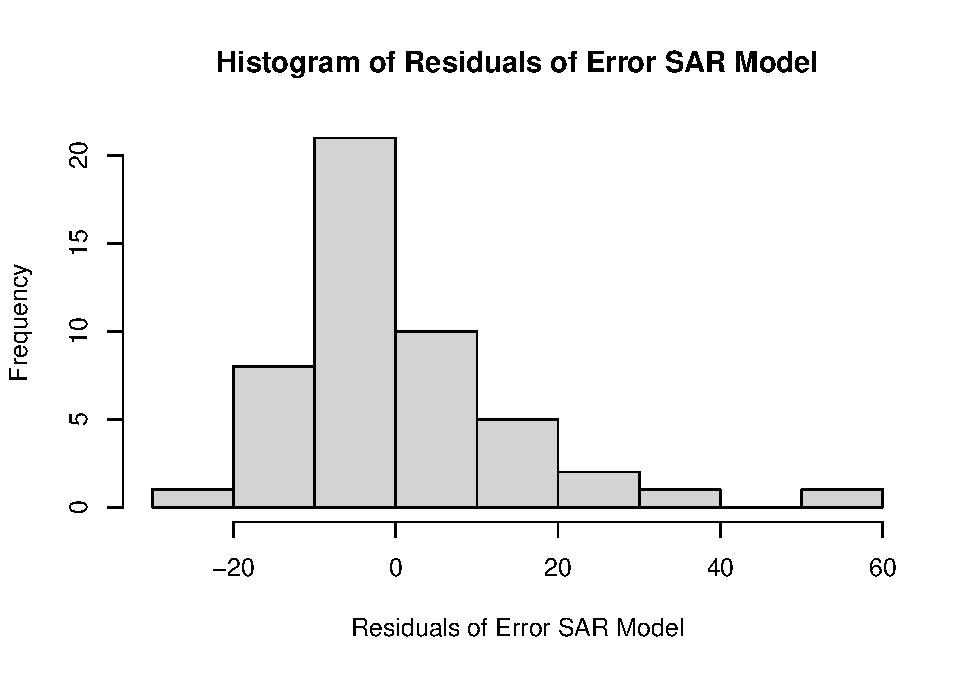
\includegraphics{midterm-project_files/figure-latex/unnamed-chunk-35-1.pdf}

The diagnostic plots suggests that the assumptions of regression are
satisfied. Yet, there might be an underlying spatial autocorrelation in
the residuals. Thus, we conduct a Moran's I test.

\(H_0\): There is no spatial autocorrelation vs \(H_1\): There is
spatial correlation. We reject \(H_0\) if the p-value
\(< \alpha = 0.05\).

\begin{Shaded}
\begin{Highlighting}[]
\CommentTok{\# Run Moran\textquotesingle{}s I test for col.lm}
\FunctionTok{moran.mc}\NormalTok{(}\FunctionTok{residuals}\NormalTok{(col.lm), lw, }\AttributeTok{nsim=}\DecValTok{499}\NormalTok{) }\CommentTok{\# significant}
\end{Highlighting}
\end{Shaded}

\begin{verbatim}
## 
##  Monte-Carlo simulation of Moran I
## 
## data:  residuals(col.lm) 
## weights: lw  
## number of simulations + 1: 500 
## 
## statistic = 0.16756, observed rank = 484, p-value = 0.032
## alternative hypothesis: greater
\end{verbatim}

Since the p-value is 0.03194, we reject \(H_0\). We conclude that there
is spatial autocorrelation in the residuals of our model.

\hypertarget{simultaneous-autoregressive-sar-error-model}{%
\subsection{Simultaneous Autoregressive (SAR) Error
Model}\label{simultaneous-autoregressive-sar-error-model}}

To address the shortcomings of the linear model under the assumption of
i.i.d. errors, we introduce \textbf{Simultaneous Autoregressive Models}.
The models solve simultaneously for the regression coefficients and for
the autoregressive error structure. In the \textbf{Spatial Error Model},
spatial autocorrelation enters in the specification only through the
error terms.

\$\$

Y\&=X beta+\varepsilon \textbackslash{} \text{where}
\quad \varepsilon\&=\lambda W \varepsilon+u \textbackslash{}
\varepsilon\&=(I-\lambda W)\^{}\{-1\} u\textbackslash{}
\therefore   \quad Y\&=X \beta+(I-\lambda W)\^{}\{-1\} u
\textbackslash{}

\$\$

where \(\mathbf{Y}\) is a vector of home values in 1000s of dollars,
\(\mathbf{X}\) is a matrix of the covariates \texttt{INC},
\texttt{CRIME}, \texttt{OPEN}, and \texttt{CP}. with constant variance
\(E\left[u u^{\prime}\right]=\sigma^{2} I\). \(\varepsilon\) is the
error term of a standard regression model, \(\lambda\) is the
autoregressive parameter, \(W\) is the row-standardised spatial weights
matrix \(W\) (that is, the weights are standardised such that
\(\Sigma_j W_{ij} = 1 \quad\text{for all}\quad i\)), and
\(u_{i} \stackrel{i.i.d.}{\sim} N(0,\sigma^2)\) a random error term.
\(I\) is the identity matrix.

In linear form the model is: \[
Y_k&=\beta_{I}Inc_{k} + \beta_{C}Crime_{k} + \beta_{O}Open_k +\beta_D DisCBD_k + \beta_{CP1} \mathbf{1}\{CP_k=1\}+\varepsilon_{k}
\]

The error variance-covariance matrix is given by

\[
E\left[\varepsilon \varepsilon^{\prime}\right]=\sigma^{2}(I-\lambda W)^{-1}\left(I-\lambda W^{\prime}\right)^{-1}
\]

In order to estimate this model, we first create a list of spatial
weights for neighbors. Then we estimate the model using the
\texttt{errorsarlm} function from the \texttt{spatialreg} package.

\begin{Shaded}
\begin{Highlighting}[]
\CommentTok{\# estimate error SAR model without transformation}
\NormalTok{col.errW.eig }\OtherTok{\textless{}{-}} \FunctionTok{errorsarlm}\NormalTok{(HOVAL}\SpecialCharTok{\textasciitilde{}}\NormalTok{INC}\SpecialCharTok{+}\NormalTok{CRIME}\SpecialCharTok{+}\NormalTok{OPEN}\SpecialCharTok{+}\FunctionTok{as.factor}\NormalTok{(CP), }\AttributeTok{data=}\NormalTok{columbus.sf,}
\NormalTok{ lw, }\AttributeTok{method=}\StringTok{"eigen"}\NormalTok{, }\AttributeTok{quiet=}\NormalTok{T)}

\CommentTok{\# look at the residuals}
\FunctionTok{hist}\NormalTok{(}\FunctionTok{residuals}\NormalTok{(col.errW.eig), }\AttributeTok{main =} \StringTok{"Histogram of Residuals of Error SAR Model"}\NormalTok{, }\AttributeTok{xlab =} \StringTok{"Residuals of Error SAR Model"}\NormalTok{)}
\end{Highlighting}
\end{Shaded}

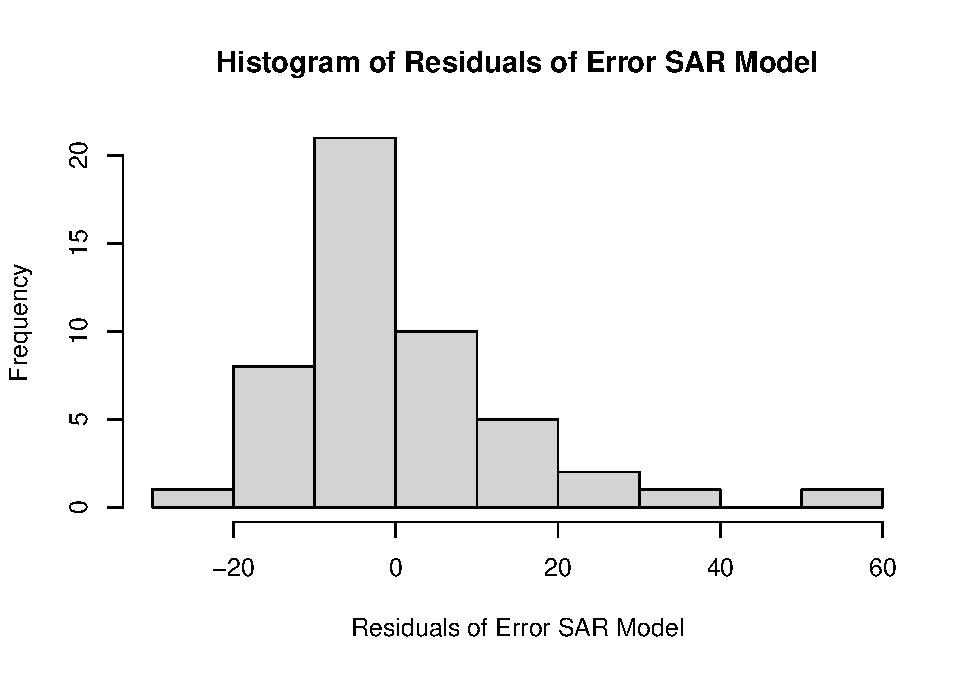
\includegraphics{midterm-project_files/figure-latex/unnamed-chunk-37-1.pdf}

The residuals are not normally distributed. We therefore, log-transform
the response to normalize them.

\begin{Shaded}
\begin{Highlighting}[]
\CommentTok{\# estimate error SAR model with log transformation}
\NormalTok{col.errW.eig.log }\OtherTok{\textless{}{-}} \FunctionTok{errorsarlm}\NormalTok{(}\FunctionTok{log}\NormalTok{(HOVAL)}\SpecialCharTok{\textasciitilde{}}\NormalTok{INC}\SpecialCharTok{+}\NormalTok{CRIME}\SpecialCharTok{+}\NormalTok{OPEN}\SpecialCharTok{+}\FunctionTok{as.factor}\NormalTok{(CP), }\AttributeTok{data=}\NormalTok{columbus.sf,}
\NormalTok{ lw, }\AttributeTok{method=}\StringTok{"eigen"}\NormalTok{, }\AttributeTok{quiet=}\NormalTok{T)}

\FunctionTok{hist}\NormalTok{(}\FunctionTok{residuals}\NormalTok{(col.errW.eig.log), }\AttributeTok{main =} \StringTok{"Histogram of Residuals of Error SAR Model (Logged Response)"}\NormalTok{, }\AttributeTok{xlab =} \StringTok{"Residuals of Error SAR Model (Logged Response)"}\NormalTok{)}
\end{Highlighting}
\end{Shaded}

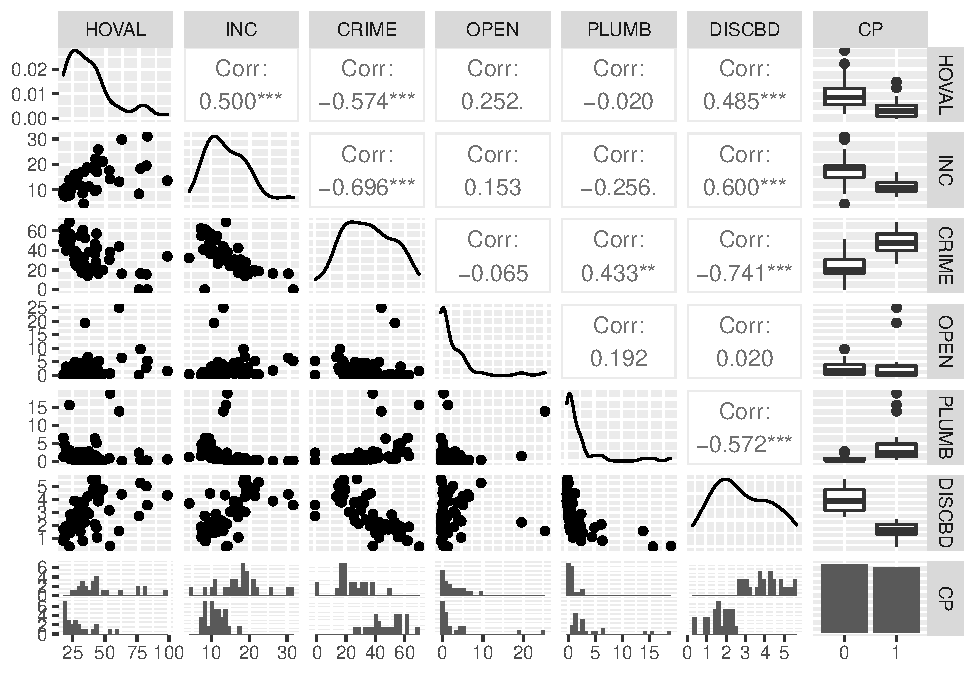
\includegraphics{midterm-project_files/figure-latex/unnamed-chunk-38-1.pdf}

\begin{Shaded}
\begin{Highlighting}[]
\CommentTok{\# print model summary}
\FunctionTok{summary}\NormalTok{(col.errW.eig.log, }\AttributeTok{correlation=}\ConstantTok{TRUE}\NormalTok{)}
\end{Highlighting}
\end{Shaded}

\begin{verbatim}
## 
## Call:errorsarlm(formula = log(HOVAL) ~ INC + CRIME + OPEN + as.factor(CP), 
##     data = columbus.sf, listw = lw, method = "eigen", quiet = T)
## 
## Residuals:
##       Min        1Q    Median        3Q       Max 
## -0.503081 -0.190516 -0.051521  0.055445  0.855101 
## 
## Type: error 
## Coefficients: (asymptotic standard errors) 
##                  Estimate Std. Error z value Pr(>|z|)
## (Intercept)     3.7832959  0.2525868 14.9782  < 2e-16
## INC             0.0134509  0.0104770  1.2839  0.19919
## CRIME          -0.0099247  0.0042443 -2.3383  0.01937
## OPEN            0.0194551  0.0086313  2.2540  0.02420
## as.factor(CP)1 -0.2520210  0.1435112 -1.7561  0.07907
## 
## Lambda: 0.45625, LR test value: 5.3082, p-value: 0.021226
## Asymptotic standard error: 0.15476
##     z-value: 2.9482, p-value: 0.0031967
## Wald statistic: 8.6916, p-value: 0.0031967
## 
## Log likelihood: -9.062429 for error model
## ML residual variance (sigma squared): 0.08037, (sigma: 0.2835)
## Number of observations: 49 
## Number of parameters estimated: 7 
## AIC: 32.125, (AIC for lm: 35.433)
## 
##  Correlation of coefficients 
##                sigma lambda (Intercept) INC   CRIME OPEN 
## lambda         -0.20                                     
## (Intercept)     0.00  0.00                               
## INC             0.00  0.00  -0.85                        
## CRIME           0.00  0.00  -0.67        0.38            
## OPEN            0.00  0.00   0.04       -0.18  0.03      
## as.factor(CP)1  0.00  0.00  -0.09        0.20 -0.50 -0.17
\end{verbatim}

We find that only \texttt{CRIME} and \texttt{OPEN} are significant at
the \(\alpha=0.05\) level. For every additional major theft (residential
burglaries and vehicle theft) per 1000 households, the predicted home
value decreases by approximately \$1010 (\(e^{0.0099247}=1.009974\)),
holding other variables constant. For every additional unit (which is
not provided in the description) of open space, the home value is
expected to increase by \$1020 (\(e^{0.0194551}=1.019646\)), holding
other variables constant.

\begin{Shaded}
\begin{Highlighting}[]
\CommentTok{\# get loglik and RMSE}
\FunctionTok{logLik}\NormalTok{(col.errW.eig.log)}
\end{Highlighting}
\end{Shaded}

\begin{verbatim}
## 'log Lik.' -9.062429 (df=7)
\end{verbatim}

\begin{Shaded}
\begin{Highlighting}[]
\FunctionTok{print}\NormalTok{(}\FunctionTok{paste0}\NormalTok{(}\StringTok{"rmse = "}\NormalTok{, }\FunctionTok{round}\NormalTok{(}\FunctionTok{sqrt}\NormalTok{(}\FunctionTok{sum}\NormalTok{((}\FunctionTok{exp}\NormalTok{(col.errW.eig.log}\SpecialCharTok{$}\NormalTok{fitted.values) }\SpecialCharTok{{-}}\NormalTok{ columbus.sf}\SpecialCharTok{$}\NormalTok{HOVAL)}\SpecialCharTok{\^{}}\DecValTok{2}\NormalTok{)), }\DecValTok{2}\NormalTok{)))}
\end{Highlighting}
\end{Shaded}

\begin{verbatim}
## [1] "rmse = 92.5"
\end{verbatim}

The log-likelihood of this model is -9.06 and the RMSE is 92.5.

We also check whether there is some spatial dependence within the
residuals of the model by performing Moran's I test. The test tests
\(H_0\): There is no spatial dependence against \(H_1\): There is
spatial dependence. We reject \(H_0\) if the test statistic
\(<\alpha=0.05\).

\begin{Shaded}
\begin{Highlighting}[]
\CommentTok{\# Run Moran\textquotesingle{}s I test for col.errW.eig.log}
\FunctionTok{moran.mc}\NormalTok{(}\FunctionTok{residuals}\NormalTok{(col.errW.eig.log), lw, }\AttributeTok{nsim=} \DecValTok{499}\NormalTok{) }\CommentTok{\# not significant}
\end{Highlighting}
\end{Shaded}

\begin{verbatim}
## 
##  Monte-Carlo simulation of Moran I
## 
## data:  residuals(col.errW.eig.log) 
## weights: lw  
## number of simulations + 1: 500 
## 
## statistic = 0.013062, observed rank = 344, p-value = 0.312
## alternative hypothesis: greater
\end{verbatim}

With a p-value of 0.3559, we fail to reject \(H_0\). There does not seem
to be any spatial dependence present in the residuals of our error
model.

log(y\_\{k\}) \mid \mu\emph{\{k\} \& \sim N\left(\mu}\{k\},
\nu\^{}\{2\}\right) \quad \text { for } k=1, \ldots, K \textbackslash{}
g\left(\mu\emph{\{k\}\right) \&=\beta}\{I\}Inc\_\{k\} +
\beta\emph{\{C\}Crime}\{k\} + \beta\emph{\{O\}Open\_k +\beta\emph{D
DisCBD\_k + \beta}\{CP1\} \mathbf{1}\{CP\_k=1\}+\psi}\{k\}

\hypertarget{conditional-autoregressive-models}{%
\subsection{Conditional Autoregressive
Models}\label{conditional-autoregressive-models}}

In the next step, we implement the conditional autoregressive (CAR)
model on the Columbus data to study the impact of covariates on House
values in Columbus, OH, 1980 with spatial information.

The CAR model essentially assumes the spatial estimation is conditional
on the value of neighbors. As a typical Bayes model, CAR model assumes
prior distribution on the model parameters and applies computationally
intensive sampling techniques like Markov Chain Monte Carlo (MCMC) or
MCMC with Gibbs sampling to find the fitted parameters.

Since we have one response variable \emph{House value}, the CAR model
has only one random effect \(\psi_k\) at each spatial location \(k\).
Because \emph{House value} is continuous, Gaussian distribution is
preferred for the CAR model and we take logarithm of the \emph{House
value} as well to make it normally distributed.

The package \emph{CARBayes} by Duncan Lee is used to apply the CAR model
in R. The specific function we use is \emph{S.CARleroux}, where it
specifies a CAR model proposed by Brian G. Leroux in 2000. The model
expression is as follows.

\$\$

log(y\_\{k\}) \mid \mu\emph{\{k\} \& \sim N\left(\mu}\{k\},
\nu\^{}\{2\}\right) \quad \text { for } k=1, \ldots, K \textbackslash{}
g\left(\mu\emph{\{k\}\right) \&=\beta}\{I\}Inc\_\{k\} +
\beta\emph{\{C\}Crime}\{k\} + \beta\emph{\{O\}Open\_k +\beta\emph{D
DisCBD\_k + \beta}\{CP1\} \mathbf{1}\{CP\_k=1\}+\psi}\{k\}

\$\$

\$\$

\psi\emph{\{k\} \mid \psi}\{-k\}, \mathbf{W}, \tau\^{}\{2\},
\rho \&\sim \mathrm{N}\left(\frac{\rho \sum_{i=1}^{K} w_{k i} \psi_{i}}{\rho \sum_{i=1}^{K} w_{k i}+1-\rho},
\frac{\tau^{2}}{\rho \sum_{i=1}^{K} w_{k i}+1-\rho}\right)
\textbackslash{} {[}\beta\_I, \beta\_C, \beta\_O, \beta\emph{D,
\beta}\{CP1\}{]}\^{}T \& \sim \mathrm{N}\left(\boldsymbol{0},
10\^{}5\boldsymbol{I}\right) \textbackslash{} \nu\^{}\{2\} \&
\sim \operatorname{Inverse-Gamma}(1, 0.01)\textbackslash{} \tau\^{}\{2\}
\& \sim \operatorname{Inverse}-\operatorname{Gamma}(1, 0.01)
\textbackslash{} \rho \& \sim \text { Uniform }(0,1)

\$\$ where

\begin{itemize}
\tightlist
\item
  \([\beta_I, \beta_C, \beta_O, \beta_D, \beta_{CP1}]^T\) are the linear
  coefficients for predictors.
\item
  \(\nu^2\) measures the variance for the logarithm of the housing
  values (\(log(y_k)\)).
\item
  \(\psi_k\) is the spatial structure component that measures the
  spatial autocorrelation.
\item
  \(\mathbf{W}\) is a neighborhood or adjacency matrix.
\item
  \(\rho\) is a spatial correlation parameter, where \(\rho=0\) means
  spatial independence and \(\rho=1\) indicates strong spatial
  correlation.
\end{itemize}

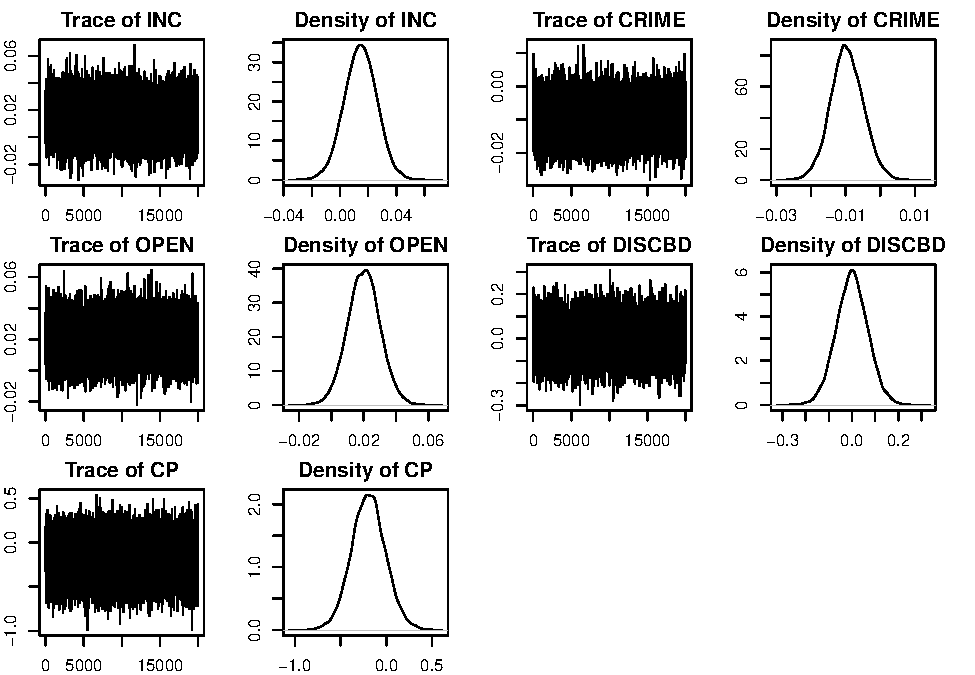
\includegraphics{midterm-project_files/figure-latex/unnamed-chunk-44-1.pdf}
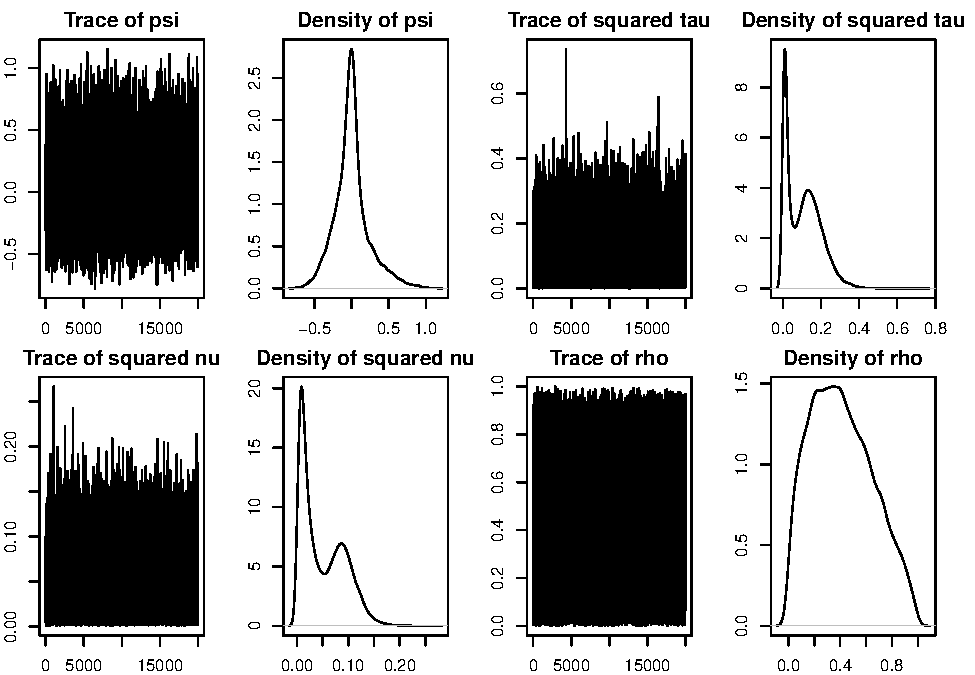
\includegraphics{midterm-project_files/figure-latex/unnamed-chunk-44-2.pdf}

\begin{longtable}[]{@{}lrrr@{}}
\caption{95\% confidence intervals for model
coefficients}\tabularnewline
\toprule
& 0.5 & 0.025 & 0.975 \\
\midrule
\endfirsthead
\toprule
& 0.5 & 0.025 & 0.975 \\
\midrule
\endhead
(Intercept) & 3.7227 & 2.9525 & 4.4936 \\
INC & 0.0147 & -0.0084 & 0.0371 \\
CRIME & -0.0097 & -0.0189 & 0.0000 \\
OPEN & 0.0201 & 0.0003 & 0.0400 \\
DISCBD & -0.0002 & -0.1345 & 0.1352 \\
CP1 & -0.1957 & -0.5607 & 0.1764 \\
\bottomrule
\end{longtable}

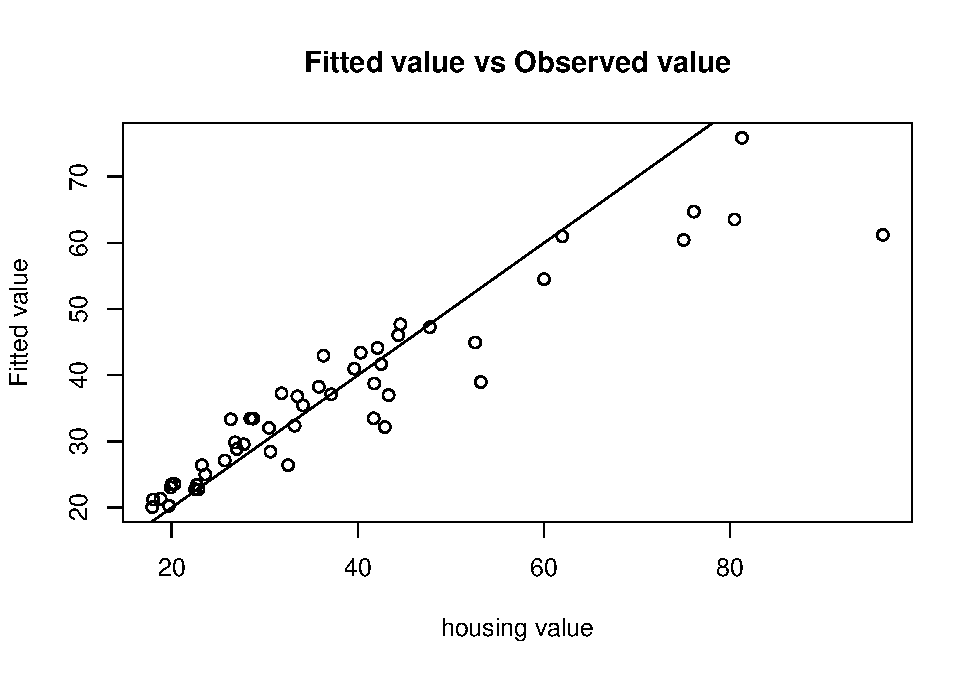
\includegraphics{midterm-project_files/figure-latex/unnamed-chunk-45-1.pdf}

The log likelihood of this model is 17.97 while the training root mean
square error (RMSE) is 52.6. From the table of \(95\%\) confidence
intervals for coefficients, we have

\begin{itemize}
\tightlist
\item
  \emph{CRIME} and \emph{OPEN} are the two variables that is significant
  since their confidence intervals don't have zero involved.
\item
  Hold other predictors fixed, regions with \textbf{less crimes} tend to
  have higher \emph{House values}.
\item
  Hold other predictors fixed, regions with \textbf{higher household
  incomes} tend to have higher \emph{House values}.
\item
  Hold other predictors fixed, regions with \textbf{more open area} tend
  to have higher \emph{House values}.
\item
  Hold other predictors fixed, regions with \textbf{closer distance to
  CBD} tend to have higher \emph{House values}.
\item
  Hold other predictors fixed, \textbf{core} regions tend to have higher
  \emph{House values}.
\end{itemize}

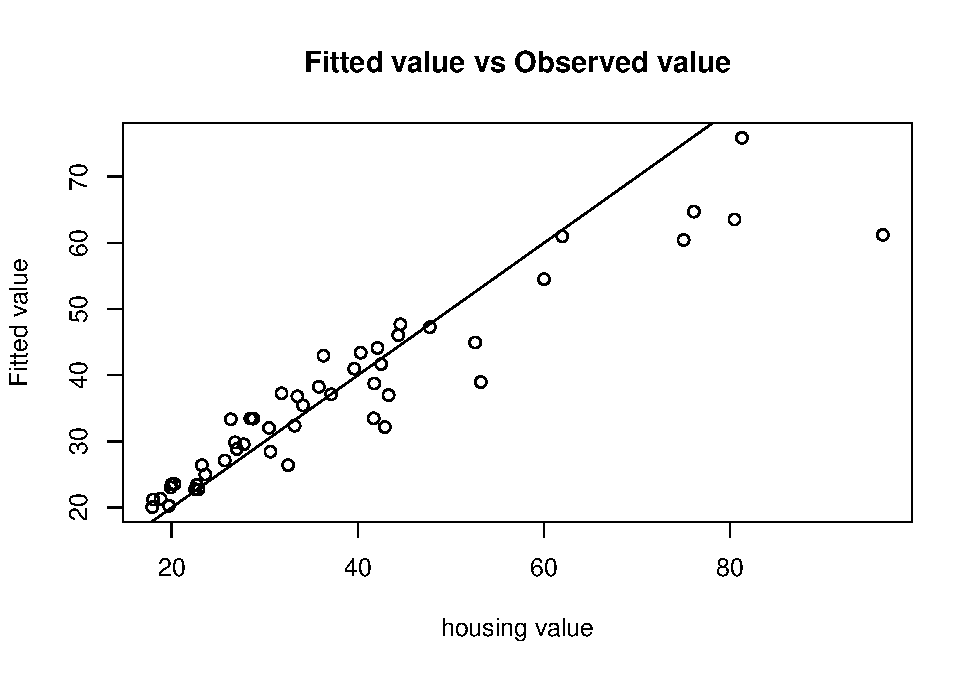
\includegraphics{midterm-project_files/figure-latex/unnamed-chunk-46-1.pdf}

\begin{Shaded}
\begin{Highlighting}[]
\CommentTok{\# Moran I}
\FunctionTok{Moran.I}\NormalTok{(}\FunctionTok{residuals}\NormalTok{(car\_model\_gaussian), ww)}\SpecialCharTok{$}\NormalTok{p.value}
\end{Highlighting}
\end{Shaded}

\begin{verbatim}
## [1] 0.09593303
\end{verbatim}

We also tested the Moran's I autocorrelation coefficient for the
residuals. It shows there is \textbf{no} significant spatial correlation
of the residuals since the p-value \(p = 0.1 > 0.05\). Therefore, our
CAR model fits the areal data nicely and leaves no significant spatial
information in the residuals.

\hypertarget{conclusions}{%
\section{Conclusions}\label{conclusions}}

From our exploratory analysis and visualizing the data we know the
variables of interest, with the exception of open space, have weak to
moderate positive spatial autocorrelation, meaning neighboring polygons
are more similar to each other than the dataset as a whole. Both the
constant mean and linear regression with i.i.d. errors had spatial
autocorrelation in their residuals. There was no spatial autocorrelation
in the SAR nor CAR models.

We found that across all of our models average house value significantly
increased with open space (units unknown). In some of the models (SAR,
CAR) housing value decreased significantly with crime (per 1000
households). In the CAR model the effect of being located in an urban
(core) neighborhood was also negative. The best fit model by log
likelihood was the CAR model.

\hypertarget{references}{%
\section*{References}\label{references}}
\addcontentsline{toc}{section}{References}

\hypertarget{refs}{}
\begin{CSLReferences}{1}{0}
\leavevmode\vadjust pre{\hypertarget{ref-R-spdep}{}}%
Bivand, Roger. 2021. \emph{Spdep: Spatial Dependence: Weighting Schemes,
Statistics}. \url{https://github.com/r-spatial/spdep/}.

\leavevmode\vadjust pre{\hypertarget{ref-sp2013}{}}%
Bivand, Roger S., Edzer Pebesma, and Virgilio Gomez-Rubio. 2013a.
\emph{Applied Spatial Data Analysis with {R}, Second Edition}. Springer,
NY. \url{https://asdar-book.org/}.

\leavevmode\vadjust pre{\hypertarget{ref-spdep2013}{}}%
---------. 2013b. \emph{Applied Spatial Data Analysis with {R}, Second
Edition}. Springer, NY. \url{https://asdar-book.org/}.

\leavevmode\vadjust pre{\hypertarget{ref-bivand2021}{}}%
Bivand, Roger, Giovanni Millo, and Gianfranco Piras. 2021. {``A Review
of Software for Spatial Econometrics in {R}.''} \emph{Mathematics} 9
(11). \url{https://doi.org/10.3390/math9111276}.

\leavevmode\vadjust pre{\hypertarget{ref-R-spData}{}}%
Bivand, Roger, Jakub Nowosad, and Robin Lovelace. 2021. \emph{spData:
Datasets for Spatial Analysis}. \url{https://nowosad.github.io/spData/}.

\leavevmode\vadjust pre{\hypertarget{ref-spdep2018}{}}%
Bivand, Roger, and David W. S. Wong. 2018. {``Comparing Implementations
of Global and Local Indicators of Spatial Association.''} \emph{TEST} 27
(3): 716--48. \url{https://doi.org/10.1007/s11749-018-0599-x}.

\leavevmode\vadjust pre{\hypertarget{ref-Furrer}{}}%
Furrer, Reinhard, and the Applied Statistics Group. 2021. {``Modeling
Dependent Data: An Excursion.''}
\url{http://user.math.uzh.ch/furrer/download/sta330/script_sta330.pdf}.

\leavevmode\vadjust pre{\hypertarget{ref-R-purrr}{}}%
Henry, Lionel, and Hadley Wickham. 2020. \emph{Purrr: Functional
Programming Tools}. \url{https://CRAN.R-project.org/package=purrr}.

\leavevmode\vadjust pre{\hypertarget{ref-R-terra}{}}%
Hijmans, Robert J. 2021. \emph{Terra: Spatial Data Analysis}.
\url{https://rspatial.org/terra/}.

\leavevmode\vadjust pre{\hypertarget{ref-R-lmtest}{}}%
Hothorn, Torsten, Achim Zeileis, Richard W. Farebrother, and Clint
Cummins. 2021. \emph{Lmtest: Testing Linear Regression Models}.
\url{https://CRAN.R-project.org/package=lmtest}.

\leavevmode\vadjust pre{\hypertarget{ref-lee2013carbayes}{}}%
Lee, Duncan. 2013. {``CARBayes: An r Package for Bayesian Spatial
Modeling with Conditional Autoregressive Priors.''} \emph{Journal of
Statistical Software} 55 (13): 1--24.

\leavevmode\vadjust pre{\hypertarget{ref-R-tibble}{}}%
Müller, Kirill, and Hadley Wickham. 2021. \emph{Tibble: Simple Data
Frames}. \url{https://CRAN.R-project.org/package=tibble}.

\leavevmode\vadjust pre{\hypertarget{ref-R-ape}{}}%
Paradis, Emmanuel, Simon Blomberg, Ben Bolker, Joseph Brown, Santiago
Claramunt, Julien Claude, Hoa Sien Cuong, et al. 2021. \emph{Ape:
Analyses of Phylogenetics and Evolution}.
\url{http://ape-package.ird.fr/}.

\leavevmode\vadjust pre{\hypertarget{ref-ape2019}{}}%
Paradis, E., and K. Schliep. 2019. {``Ape 5.0: An Environment for Modern
Phylogenetics and Evolutionary Analyses in {R}.''} \emph{Bioinformatics}
35: 526--28.

\leavevmode\vadjust pre{\hypertarget{ref-sf2018}{}}%
Pebesma, Edzer. 2018. {``{Simple Features for R: Standardized Support
for Spatial Vector Data}.''} \emph{{The R Journal}} 10 (1): 439--46.
\url{https://doi.org/10.32614/RJ-2018-009}.

\leavevmode\vadjust pre{\hypertarget{ref-R-sf}{}}%
---------. 2021. \emph{Sf: Simple Features for r}.
\url{https://CRAN.R-project.org/package=sf}.

\leavevmode\vadjust pre{\hypertarget{ref-sp2005}{}}%
Pebesma, Edzer J., and Roger S. Bivand. 2005. {``Classes and Methods for
Spatial Data in {R}.''} \emph{R News} 5 (2): 9--13.
\url{https://CRAN.R-project.org/doc/Rnews/}.

\leavevmode\vadjust pre{\hypertarget{ref-R-sp}{}}%
Pebesma, Edzer, and Roger Bivand. 2021. \emph{Sp: Classes and Methods
for Spatial Data}. \url{https://CRAN.R-project.org/package=sp}.

\leavevmode\vadjust pre{\hypertarget{ref-R-base}{}}%
R Core Team. 2021. \emph{R: A Language and Environment for Statistical
Computing}. Vienna, Austria: R Foundation for Statistical Computing.
\url{https://www.R-project.org/}.

\leavevmode\vadjust pre{\hypertarget{ref-R-GGally}{}}%
Schloerke, Barret, Di Cook, Joseph Larmarange, Francois Briatte, Moritz
Marbach, Edwin Thoen, Amos Elberg, and Jason Crowley. 2021.
\emph{GGally: Extension to Ggplot2}.
\url{https://CRAN.R-project.org/package=GGally}.

\leavevmode\vadjust pre{\hypertarget{ref-ver2018relationship}{}}%
Ver Hoef, Jay M, Ephraim M Hanks, and Mevin B Hooten. 2018. {``On the
Relationship Between Conditional (CAR) and Simultaneous (SAR)
Autoregressive Models.''} \emph{Spatial Statistics} 25: 68--85.

\leavevmode\vadjust pre{\hypertarget{ref-ggplot22016}{}}%
Wickham, Hadley. 2016. \emph{Ggplot2: Elegant Graphics for Data
Analysis}. Springer-Verlag New York.
\url{https://ggplot2.tidyverse.org}.

\leavevmode\vadjust pre{\hypertarget{ref-R-stringr}{}}%
---------. 2019. \emph{Stringr: Simple, Consistent Wrappers for Common
String Operations}. \url{https://CRAN.R-project.org/package=stringr}.

\leavevmode\vadjust pre{\hypertarget{ref-R-forcats}{}}%
---------. 2021a. \emph{Forcats: Tools for Working with Categorical
Variables (Factors)}. \url{https://CRAN.R-project.org/package=forcats}.

\leavevmode\vadjust pre{\hypertarget{ref-R-tidyr}{}}%
---------. 2021b. \emph{Tidyr: Tidy Messy Data}.
\url{https://CRAN.R-project.org/package=tidyr}.

\leavevmode\vadjust pre{\hypertarget{ref-R-tidyverse}{}}%
---------. 2021c. \emph{Tidyverse: Easily Install and Load the
Tidyverse}. \url{https://CRAN.R-project.org/package=tidyverse}.

\leavevmode\vadjust pre{\hypertarget{ref-tidyverse2019}{}}%
Wickham, Hadley, Mara Averick, Jennifer Bryan, Winston Chang, Lucy
D'Agostino McGowan, Romain François, Garrett Grolemund, et al. 2019.
{``Welcome to the {tidyverse}.''} \emph{Journal of Open Source Software}
4 (43): 1686. \url{https://doi.org/10.21105/joss.01686}.

\leavevmode\vadjust pre{\hypertarget{ref-R-ggplot2}{}}%
Wickham, Hadley, Winston Chang, Lionel Henry, Thomas Lin Pedersen,
Kohske Takahashi, Claus Wilke, Kara Woo, Hiroaki Yutani, and Dewey
Dunnington. 2021. \emph{Ggplot2: Create Elegant Data Visualisations
Using the Grammar of Graphics}.
\url{https://CRAN.R-project.org/package=ggplot2}.

\leavevmode\vadjust pre{\hypertarget{ref-R-dplyr}{}}%
Wickham, Hadley, Romain François, Lionel Henry, and Kirill Müller. 2021.
\emph{Dplyr: A Grammar of Data Manipulation}.
\url{https://CRAN.R-project.org/package=dplyr}.

\leavevmode\vadjust pre{\hypertarget{ref-R-readr}{}}%
Wickham, Hadley, and Jim Hester. 2021. \emph{Readr: Read Rectangular
Text Data}. \url{https://CRAN.R-project.org/package=readr}.

\leavevmode\vadjust pre{\hypertarget{ref-zoo2005}{}}%
Zeileis, Achim, and Gabor Grothendieck. 2005. {``Zoo: S3 Infrastructure
for Regular and Irregular Time Series.''} \emph{Journal of Statistical
Software} 14 (6): 1--27. \url{https://doi.org/10.18637/jss.v014.i06}.

\leavevmode\vadjust pre{\hypertarget{ref-R-zoo}{}}%
Zeileis, Achim, Gabor Grothendieck, and Jeffrey A. Ryan. 2021.
\emph{Zoo: S3 Infrastructure for Regular and Irregular Time Series (z's
Ordered Observations)}. \url{https://zoo.R-Forge.R-project.org/}.

\leavevmode\vadjust pre{\hypertarget{ref-lmtest2002}{}}%
Zeileis, Achim, and Torsten Hothorn. 2002. {``Diagnostic Checking in
Regression Relationships.''} \emph{R News} 2 (3): 7--10.
\url{https://CRAN.R-project.org/doc/Rnews/}.

\end{CSLReferences}

\end{document}
